\documentclass[conference, 12pt]{IEEEtran}

\usepackage{cite}						% Used to create bibliography
\usepackage{amsmath, amssymb, amsfonts}	% Used to create equations and math statements
\usepackage{algorithmic}				
\usepackage{graphicx}					% Used to attach images
\usepackage{float}						% Used to move images around
\usepackage{siunitx}					% Used to display mu in non-math mode
\usepackage[top=1in, right=1in, left=1in, bottom=1in]{geometry}

\newcommand{\x}{1}						% Create width of images
\newcommand{\figPos}{tbp}				% Place figures at top or bottom of columns

\begin{document}
	% Create title, author, and date information
	\title{Differential Power Analysis Resistant Cryptographic Circuits}
	\author{\IEEEauthorblockN{Nicholas Chiapputo}
	\IEEEauthorblockA{EENG 4710.001}}
	\date{23 October 2019}

	\maketitle
	
	\section{Introduction}
		Side channel attacks target cryptographic devices and retrieve unintentionally leaked information in the form of power, electromagnetic radiation, or operation timing. Adversaries can mount these attacks to retrieve plaintext, ciphertext, and keys to read confidential information and compromise supposedly secure cryptographic algorithms. As adversarial power increases, limiting attack vectors becomes increasingly important to secure data. Solutions to this problem have applications wherever data security is necessary including mobile devices in Internet of Things (IoT), military and government applications, as well as common applications such as web traffic and peer-to-peer communications.

		The most popular and powerful side channel attack is known as power analysis. In power analysis, the adversary gains full control over the circuit, its inputs, and its outputs and measures current, or power, through the resistor. This information can then be analyzed to find sources of information leakage either through the design of the algorithm, the logic gates, or the transistors themselves. Differential Power Analysis (DPA) is a very powerful method of attack first proposed in \cite{b7}. This attack analyzes the power traces of the circuit statistically to find sources of information leakage that may otherwise have been very difficult to spot using traditional analysis. 

		Many logic families have been proposed to solve this problem and replace the normal CMOS logic design which tends to leak significant amounts of information. The most popular logic style uses differential logic. Significant logic families using this style are Three-Phase Dual-Rail Pre-Charge Logic (TDPL) and Sense Amplifier Based Logic (SABL) which use differential logic to perform logical operations while consuming a constant amount of energy. 

		Current Mode Logic (CML) is also used to increase the switching speed of the process while using a constant current input. This logic can further be improved by using emerging technologies such as Tunnel FETs (TFETs) or Silicon Nano-Wire FETS (SiNWFETs) to reduce the power consumption and threshold voltage. 

		Section II introduces the Differential Power Analysis attack is explained and Section III discusses current proposed solutions to the attack. Section IV then compares the performance and power consumption of each of the proposed solutions and Section V concludes the report. 


	\section{Differential Power Analysis}
		The most basic power analysis attack on cryptographic circuits is Simple Power Analysis (SPA). In this attack, the adversary is assumed to have unlimited access to the device as well as control over the plaintext and key input. To mount the attack, the adversary attaches a resistance, usually 50Ω, in series with either the voltage source or ground reference. Probes are then attached to the device to measure current or power through the resistor and a single cryptographic operation is run through the circuit with a chosen plaintext (or ciphertext) and key input. The adversary can then analyze this single power trace for information leakage clues. Figure \ref{SPA} shows an example SPA trace. 

		\begin{figure}[tbp]
			\centering
			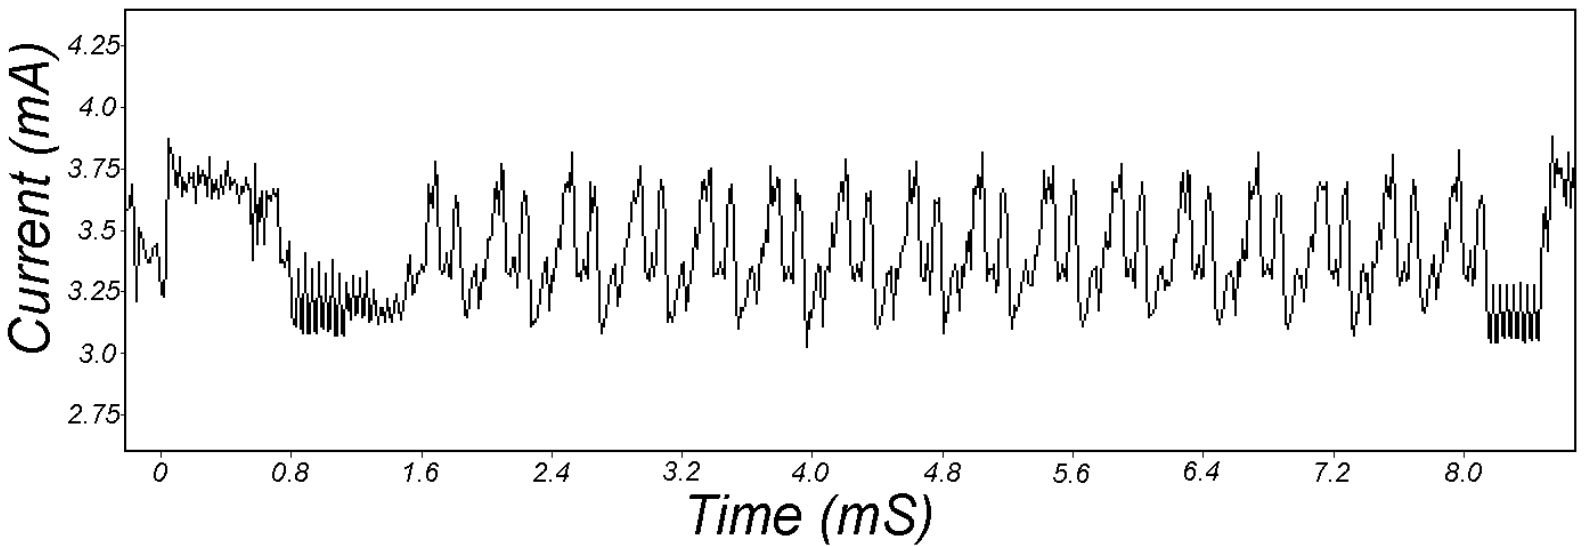
\includegraphics[width=\x\linewidth]{ReportFiles/SPA.png}
			\caption{SPA trace of one DES operation.\cite{b7}}
			\label{SPA}
		\end{figure}

		While this attack can give some information such as the encryption/decryption algorithm being used as well as timing information for some operations, it is generally trivial to counter and is a generally weak attack. In \cite{b7}, Differential Power Analysis (DPA) is first introduced. In this new attack, the adversary is assumed to have the same abilities (unlimited device access, plaintext/key/ciphertext control). Instead of one power trace, multiple traces (normally 10,000) are taken with a large number of samples (normally 100,000). 

		A selection function $D(C, b K_s)$ is defined to compute the value of the $b^{th}$ bit of the guessed key $K_s$ corresponding to the output ciphertext $C$. The output of the selection value is either 0 or 1, representing the $b^{th}$ bit value. Once the power traces are taken, they are separated into groups based on the binary output of the selection function $D$. These two sets are then averaged within themselves to calculate the average power traces $A_0$ and $A_1$. The difference $\Delta D = A_0-A_1$ is calculated to represent the average effect of the selection function on the total power consumption. 

		This differential power trace is plotted for each key bit value, or a sufficient number of bits before a simple computational attack can be carried out. Figure \ref{DPA} shows an example DPA attack. The topmost trace is a reference power trace showing the average power consumption of a single DES operation. The second trace shows a large spike, indicating that the guessed key Ks is correct while the lower two show no more than general noise indicating that the guessed keys are incorrect. 

		\begin{figure}[tbp]
			\centering
			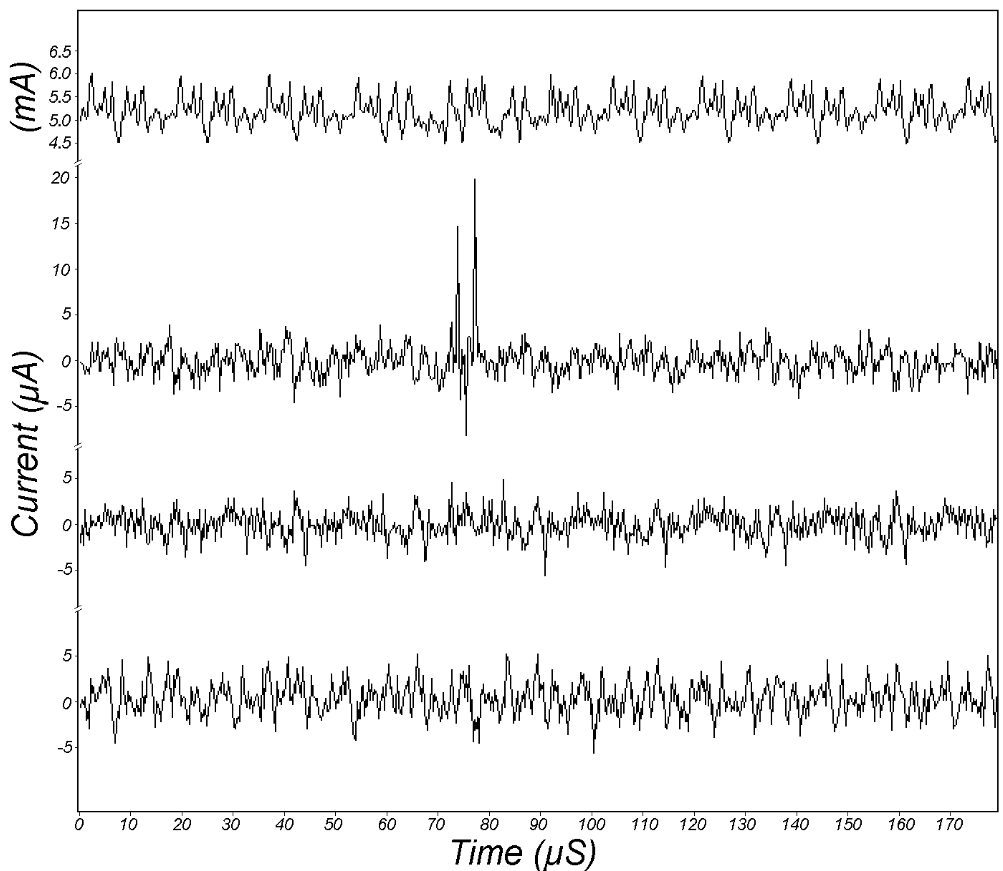
\includegraphics[width=\x\linewidth]{ReportFiles/DPA.png}
			\caption{DPA power traces with reference DES trace (top), correct key guess (second from top), and two incorrect key guesses (bottom two).\cite{b7}}
			\label{DPA}
		\end{figure}

		To further reduce noise and achieve a more clear outcome, an increasing number of samples can be taken. Using this, it can be seen that many common power analysis countermeasures, such as the introduction of random noise or redundant data, may not be very effective against the much more powerful DPA attack. Instead, more intensive measures must be taken to ensure adversaries can not find information leakage regardless of the number of samples or traces that are taken.

	\section{Countermeasures to DPA}
		Given that DPA makes use of the difference between two average power traces, its effectiveness can be limited by reducing the power deviation of the cryptographic circuit. This value is generally referred to as the energy deviation of a circuit and can be calculated by taking the average energy trace of each input combination and comparing how the energy consumption varies for each case. Since any new implementations are being compared to CMOS logic styles, Normalized Energy Deviation (NED) is used to compare performance. In this measurement, the NED of proposed DPA-resistant circuits is calculated as a percentage of CMOS logic which is the normalized value of 100%.

		To achieve perfect security by limiting information leakage through DPA, a constant power output is needed. With this, the differential power traces will always be zero, regardless of the input value, rendering any power analysis technique useless. However, this is very difficult to do in practice with non-ideal scenarios that exist in real-world applications. In general, a 1\% NED is considered to be adequately secure against DPA attacks.

		Many proposed logic styles use differential logic to ensure that the switching power of a gate will be constant as each input and output line switches exactly twice per calculation, thereby reducing the NED. With this, however, comes significant extra power usage. While not much research has been done towards limiting this, emerging technologies replacing MOSFETs have been shown to theoretically reduce the power consumption of not only DPA-resistant circuits, but also traditional CMOS logic style circuits.


		\subsection{Three-Phase Dual-Rail Pre-Charge Logic}
			Differential logic styles such as Three-Phase Dual-Rail Pre-Charge Logic (TDPL) are among the most researched DPA-resistant logic families. Due to its differential nature, TDPL has a low NED, making it a strong competitor against DPA. The dual-rail characteristic of TDPL means that every output of the cell is complementary. That is, for logic gates with output values 0 and 1, the output lines are $out$ and $\overline{out}$. 

			The first part of the name, Three-Phase, references the three internal phases TDPL goes through in order to ensure all output and input lines transition from 1 to 0 and 0 to 1 every clock cycle to ensure a constant energy consumption. These three-phases, in the standard implementation from \cite{b1}, are sourced from three external clock sources.

			The first phase is known as the pre-charge phase. In this phase, the differential output values $out$ and $\overline{out}$ are discharged to 0. In the following evaluation phase, the appropriate output line is set high depending on the input values. The third phase, added in this proposed logic style, charges the other output line to $V_{DD}$ so that both output lines end high, ensuring that there is a 0 to 1 and 1 to 0 transition for both lines during each cycle. The timing diagram for a TDPL NAND/AND gate is included in Figure \ref{TDPL_NAND_Timing} and the NAND/AND implementation from \cite{b1} is in Figure \ref{TDPL_NAND}.

			\begin{figure}[tbp]
				\centering
				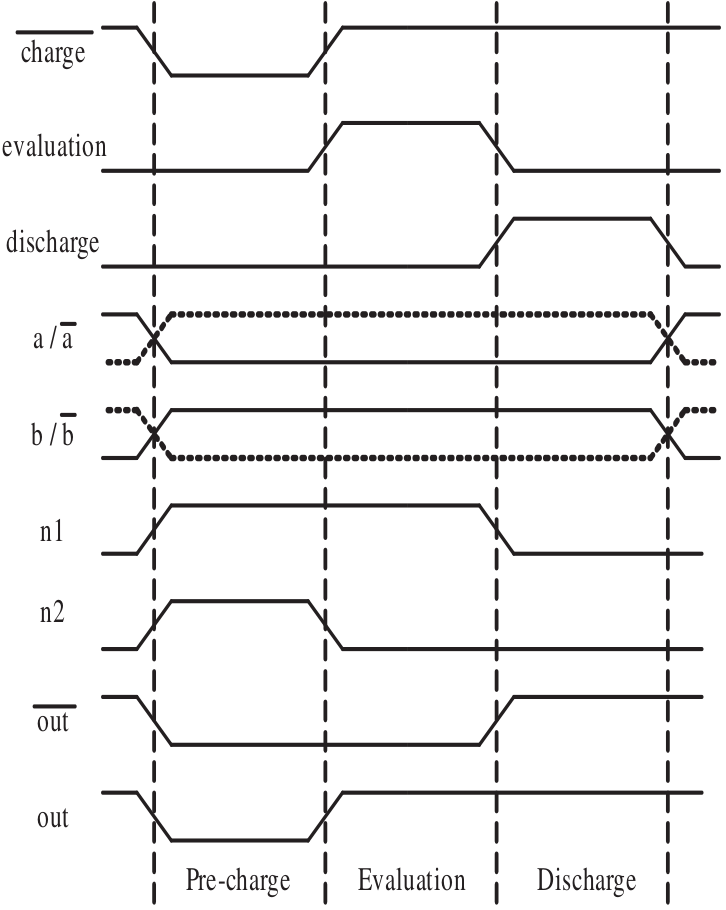
\includegraphics[width=\x\linewidth]{ReportFiles/TDPL_NAND_Timing.png}
				\caption{TDPL NAND/AND gate timing diagram.\cite{b1}}
				\label{TDPL_NAND_Timing}
			\end{figure}
			\begin{figure}[tbp]
				\centering
				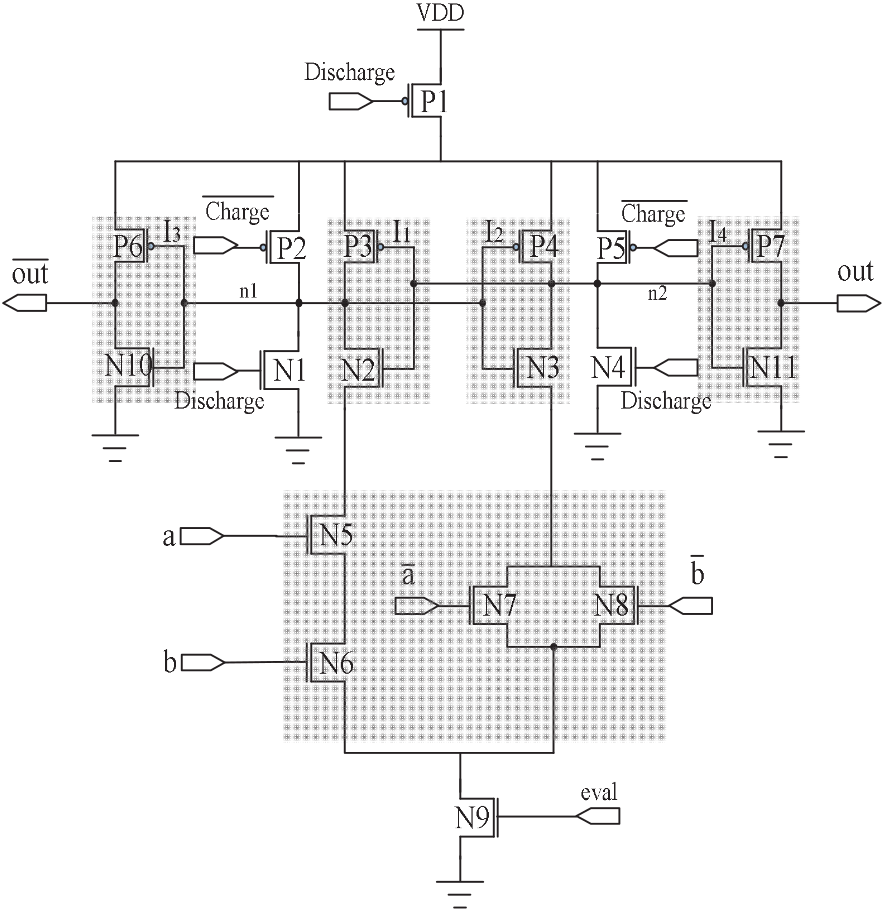
\includegraphics[width=\x\linewidth]{ReportFiles/TDPL_NAND.png}
				\caption{TDPL NAND/AND gate circuit schematic.\cite{b1}}
				\label{TDPL_NAND}
			\end{figure}

			In \cite{b1}, TDPL and CMOS logic styles are used to implement a cryptographic s-box used for key permutation in various cryptographic algorithms. Then, DPA attacks are carried out on both implementations to show that TDPL uses a constant amount of power for each stage while CMOS uses varying power based on the operations and switches that occur during each computation. Figure \ref{CMOS_S-box_Power} shows the CMOS power trace and Figure \ref{TDPL_S-box_Power} shows the constant power output of the TDPL implementation.

			\begin{figure}[tbp]
				\centering
				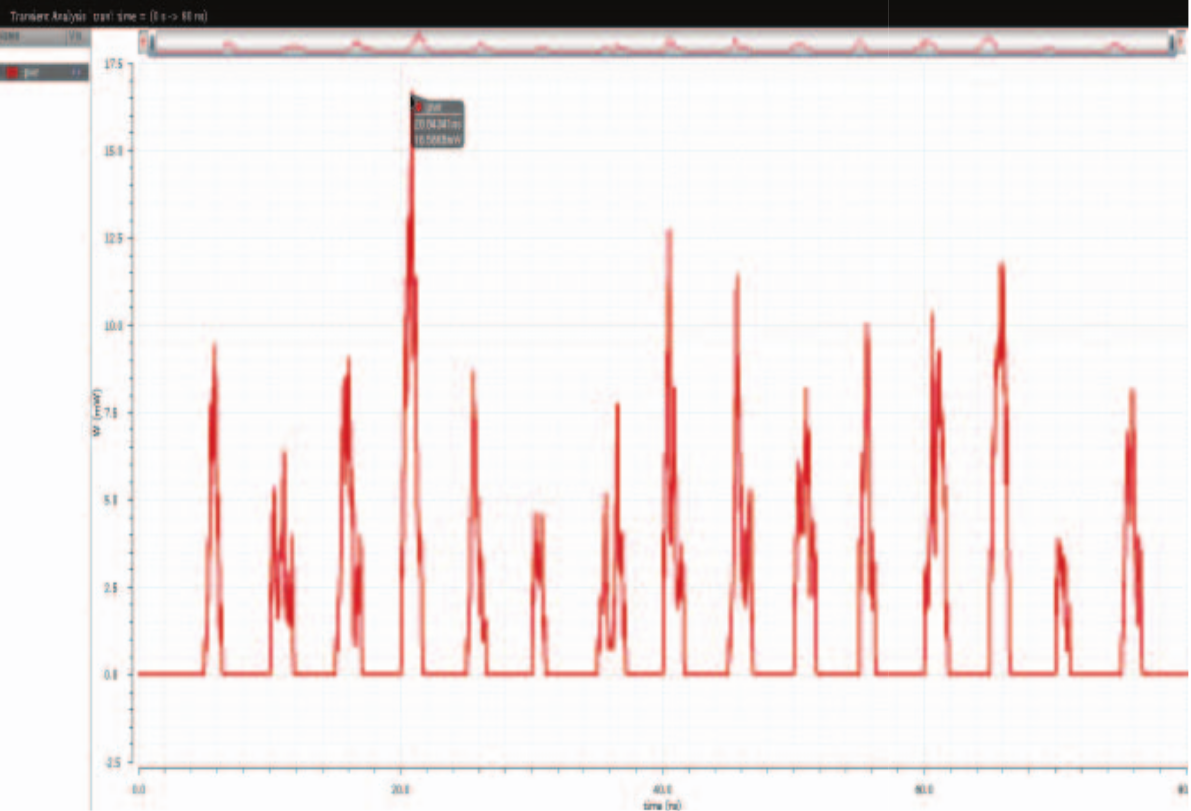
\includegraphics[width=\x\linewidth]{ReportFiles/CMOS_S-box_Power.png}
				\caption{CMOS power trace from S-box 6 implementation.\cite{b1}}
				\label{CMOS_S-box_Power}
			\end{figure}

			\begin{figure}[tbp]
				\centering
				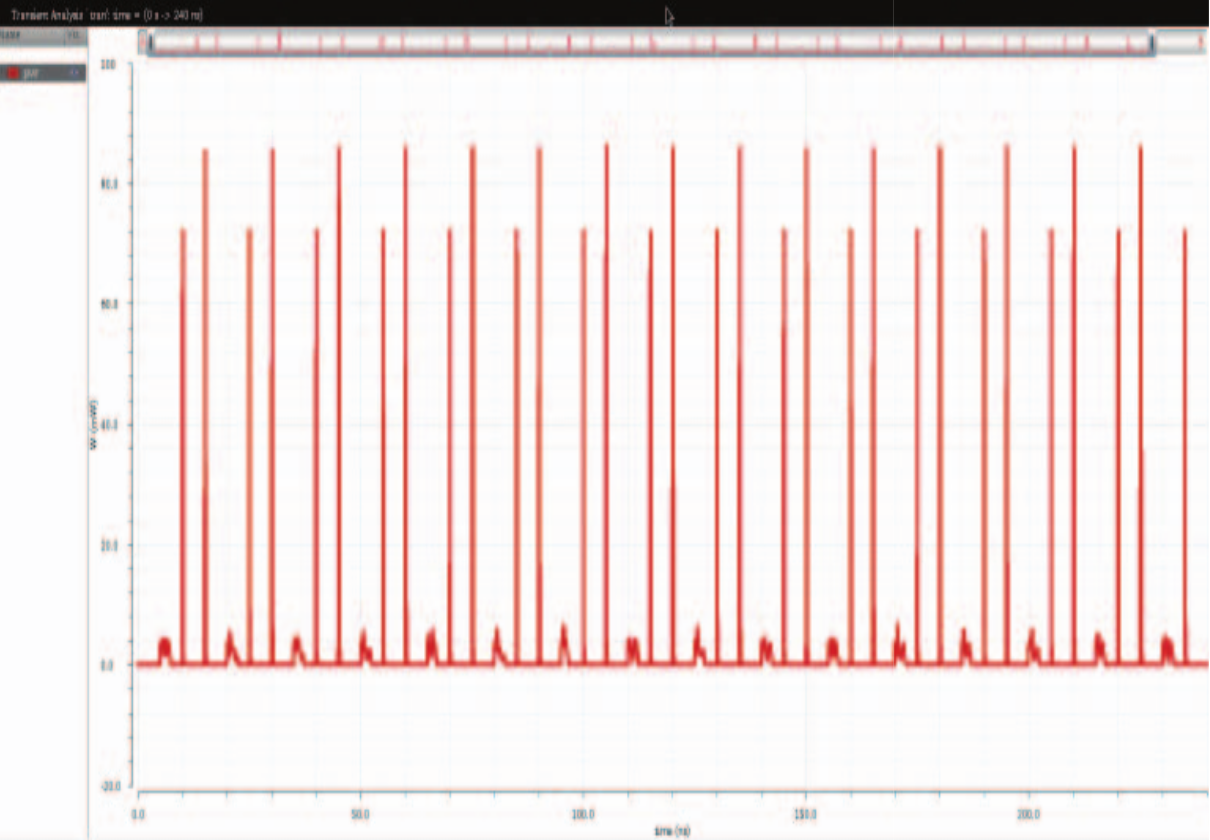
\includegraphics[width=\x\linewidth]{ReportFiles/TDPL_S-box_Power.png}
				\caption{TDPL power trace showing constant power in S-box 6 implementation.\cite{b1}}
				\label{TDPL_S-box_Power}
			\end{figure}

			Reference \cite{b2} expands upon this implementation by introducing a timing attack. In this proposed attack, the adversary gains control of the clock that is external to the TDPL gate and is able to slow down the clocks to stretch out the individual phases, allowing the adversary a clearer view of the switching power being consumed. This attack can be expanded to allow the adversary to completely cut out the clock during the discharge phase by grounding the discharge clock source, thereby allowing a DPA attack to be successful as one of the output lines will now only switch once, creating a difference in consumed switching power. This then reduces the energy deviation, reducing the number of power traces an adversary needs before the DPA attack is successful.

			To counter this, the authors propose Self-Timed TDPL (ST-TDPL) which includes a single clock source with only one phase. The three phases of TDPL execution are then generated internally. The pre-charge phase occurs in the first half of the clock period while the clock signal is low.The evaluation phase occurs in the second half while the clock signal is high. In ST-TDPL implementation, the logic gates are connected in order of stages where each stage sends a signal, DONE, back to the previous stage. The DONE signal is calculated simply as the NAND of two internal line signals $X$ and $Y$ as shown in the ST-TDPL NAND schematic in Figure \ref{ST-TDPL_NAND}.

			\begin{figure}[tbp]
				\centering
				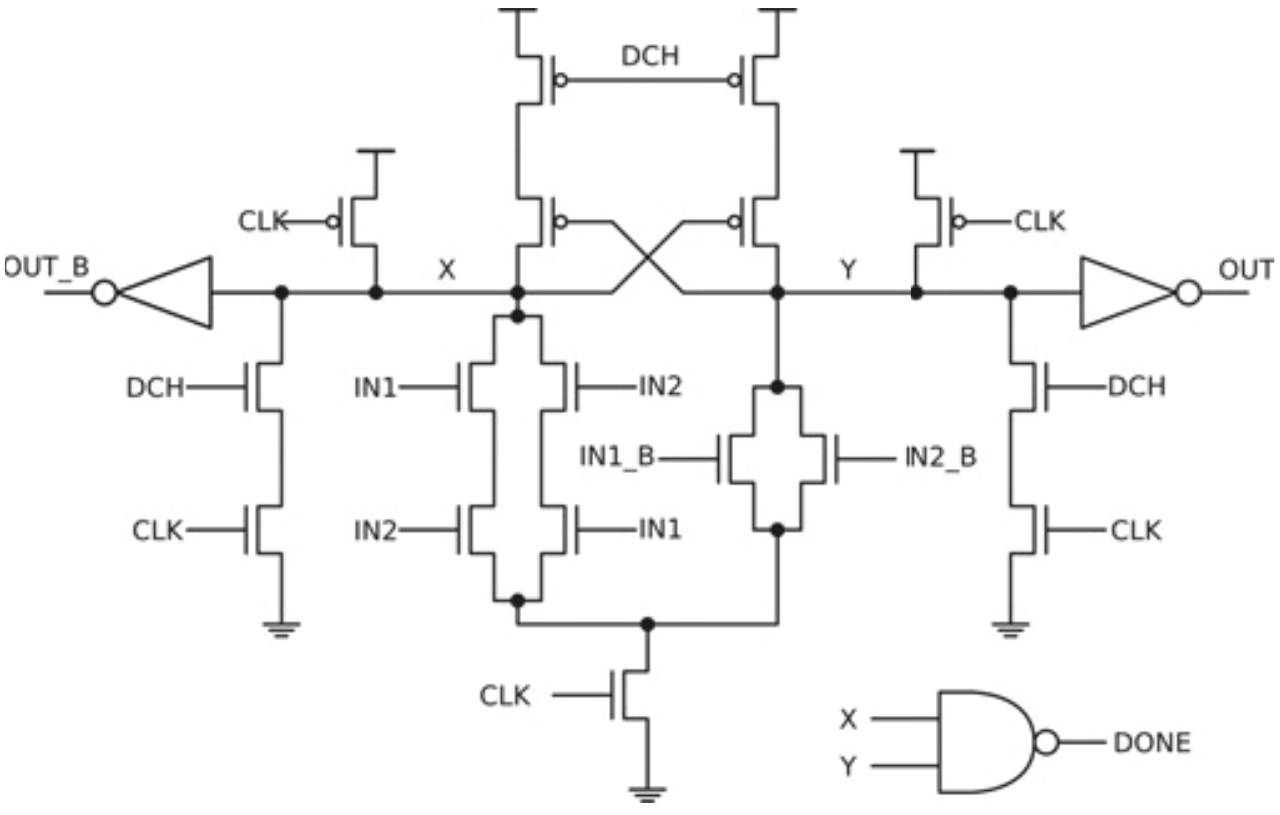
\includegraphics[width=\x\linewidth]{ReportFiles/ST-TDPL_NAND.png}
				\caption{ST-TDPL NAND gate schematic.\cite{b2}}
				\label{ST-TDPL_NAND}
			\end{figure}

			The discharge phase is then triggered asynchronously with the use of the DONE signal. An example chain of ST-TDPL inverter gates is shown in Figure \ref{ST-TDPL_INV_Chain} and the timing diagram of a NAND gate is shown in Figure \ref{ST-TDPL_NAND_Timing}.

			\begin{figure}[tbp]
				\centering
				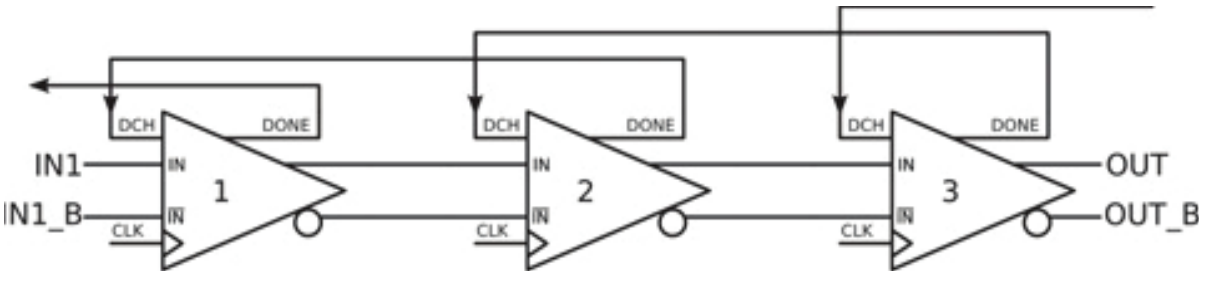
\includegraphics[width=\x\linewidth]{ReportFiles/ST-TDPL_INV_Chain.png}
				\caption{ST-TDPL inverter gate chaining.\cite{b2}}
				\label{ST-TDPL_INV_Chain}
			\end{figure}

			\begin{figure}[tbp]
				\centering
				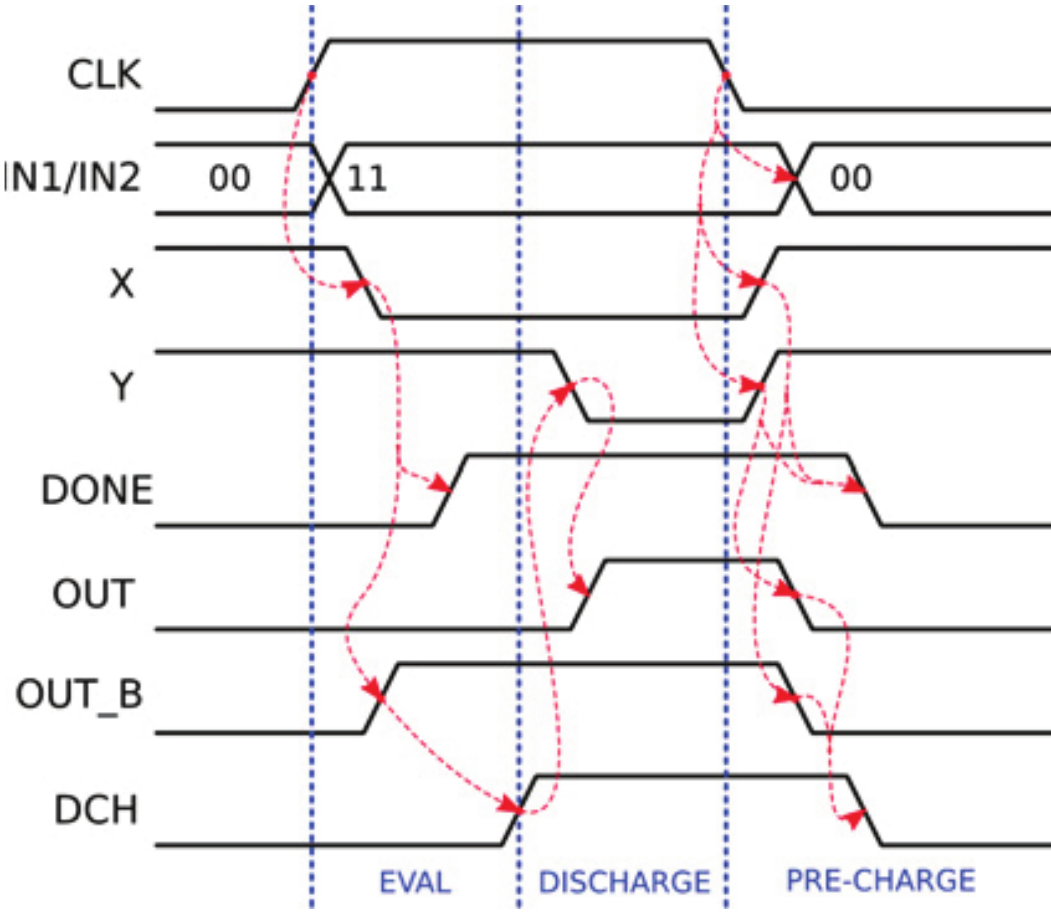
\includegraphics[width=\x\linewidth]{ReportFiles/ST-TDPL_NAND_Timing.png}
				\caption{ST-TDPL NAND timing diagram.\cite{b2}}
				\label{ST-TDPL_NAND_Timing}
			\end{figure}

			Comparing the improved design of Figure \ref{ST-TDPL_NAND} with the original TDPL design in Figure \ref{TDPL_NAND}, it can be seen that the internal lines $X$ ($n1$ in TDPL) and $Y$ ($n2$ in TDPL) are gated using a PMOS with the gate connected to the clock signal. Additionally, the discharge devices are gated using an NMOS with the gate connected to the clock signal. This design choice prevents a drive fight between the discharge and the evaluation stages where the discharge device is attempting to discharge the final internal line while the evaluation device is still attempting to charge one of these lines. 

			This issue can be seen in the TDPL timing diagram of Figure \ref{TDPL_NAND_Timing} where $n1$ is switching on the rising edge of the discharge signal. Comparing this with the ST-TDPL timing diagram of Figure \ref{ST-TDPL_NAND_Timing}, it can be seen that there is no longer any drive fight between these two phases as the signal $Y$ does not discharge until after the evaluation stage is completely done and the discharge signal is fully on.

			Because of this improvement, there is significantly less power loss during the phase change, thereby decreasing the normalized energy consumption as shown in Figure \ref{ST-TDPL_Energy} where CMOS, TDPL, compromised TDPL (adversary has disabled the discharge clock), and ST-TDPL energy consumption is compared. Additionally, the Normalized Energy Deviation (NED) of ST-TDPL is marginally better than standard TDPL. Figure \ref{ST-TDPL_NED} shows the NED comparisons between CMOS, TDPL, compromised TDPL, and ST-TDPL implementations.

			\begin{figure}[tbp]
				\centering
				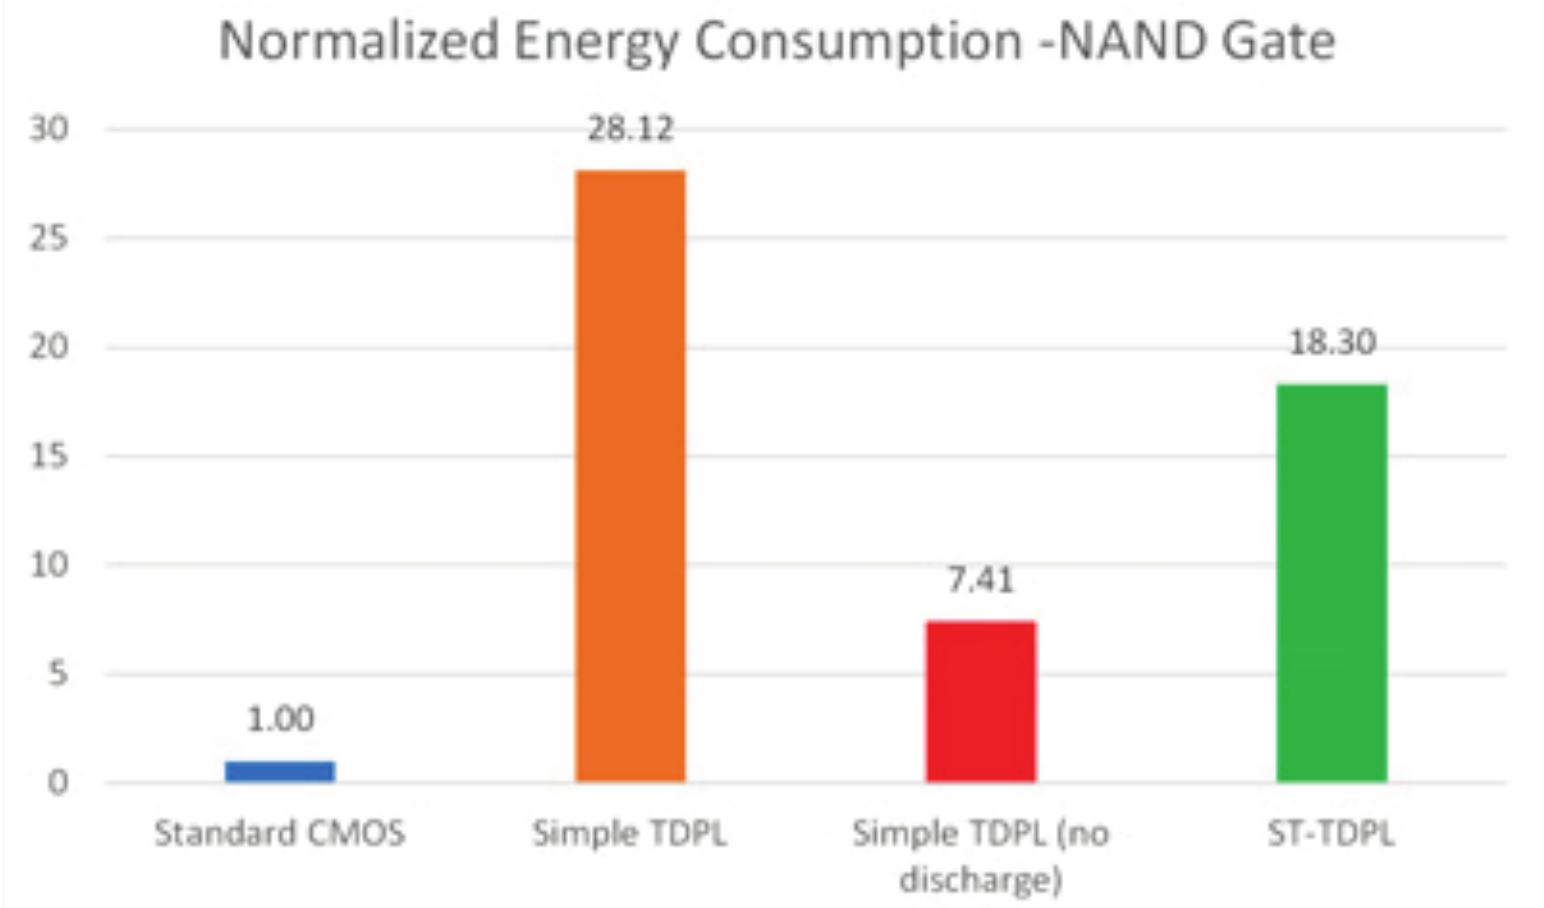
\includegraphics[width=\x\linewidth]{ReportFiles/ST-TDPL_Energy.png}
				\caption{NAND gate energy consumption for CMOS, TDPL, compromised TDPL, and ST-TDPL.\cite{b2}}
				\label{ST-TDPL_Energy}
			\end{figure}

			\begin{figure}[tbp]
				\centering
				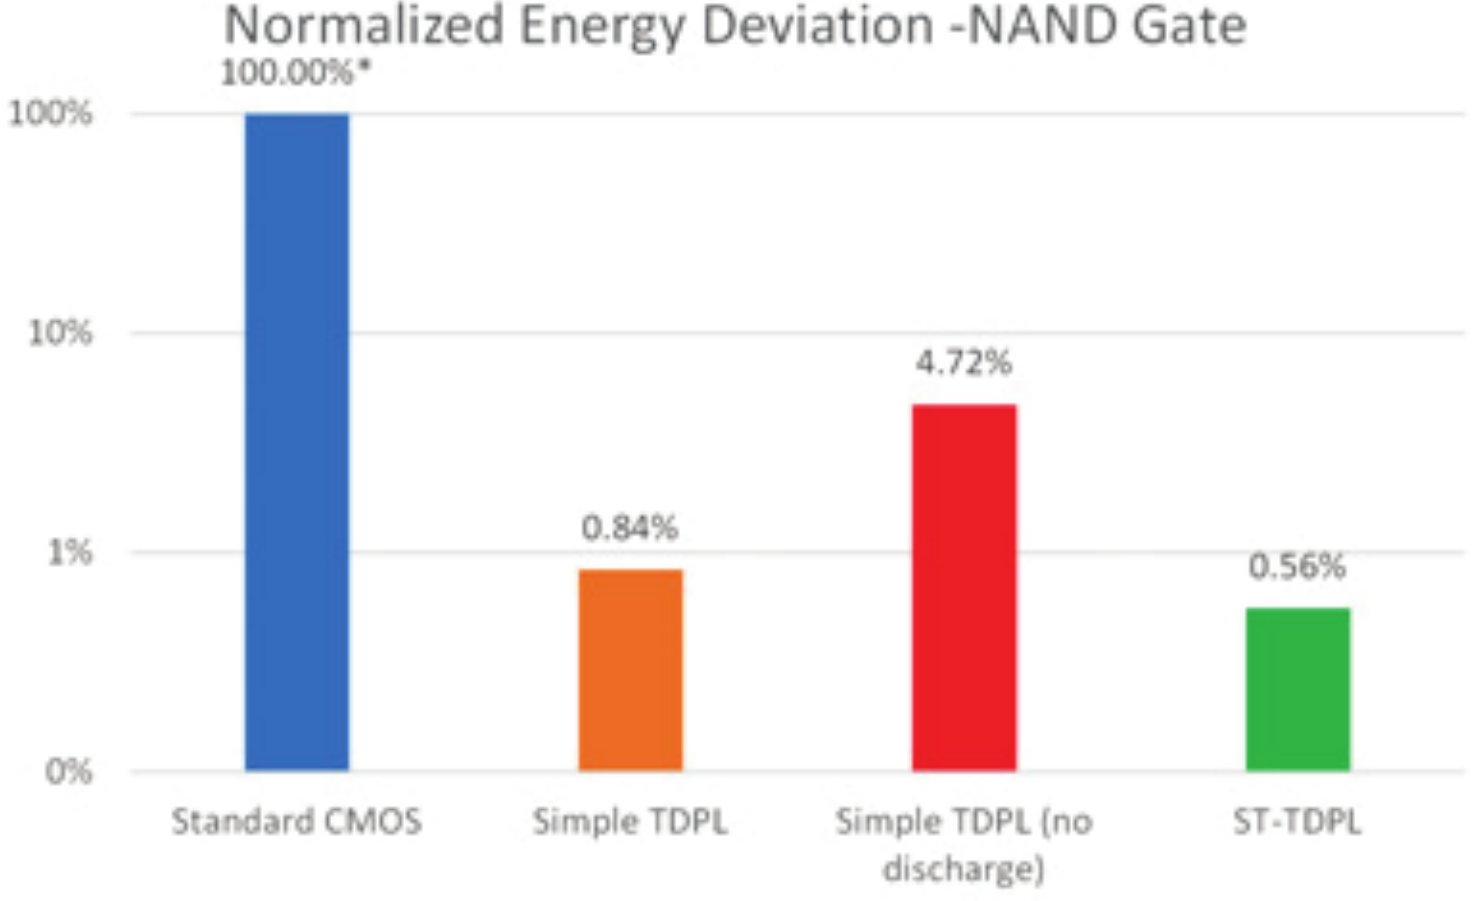
\includegraphics[width=\x\linewidth]{ReportFiles/ST-TDPL_NED.png}
				\caption{NAND gate NED for CMOS, TDPL, compromised TDPL, and ST-TDPL.\cite{b2}}
				\label{ST-TDPL_NED}
			\end{figure}

			Due to the additional logic of the DONE signal as well as the gating of the evaluation and discharge phases, there is some area overhead. This additional cost, however, is not very significant in comparison to the significant energy savings of ST-TDPL. The gate area comparisons can be seen in Figure \ref{ST-TDPL_Area}.

			\begin{figure}[tbp]
				\centering
				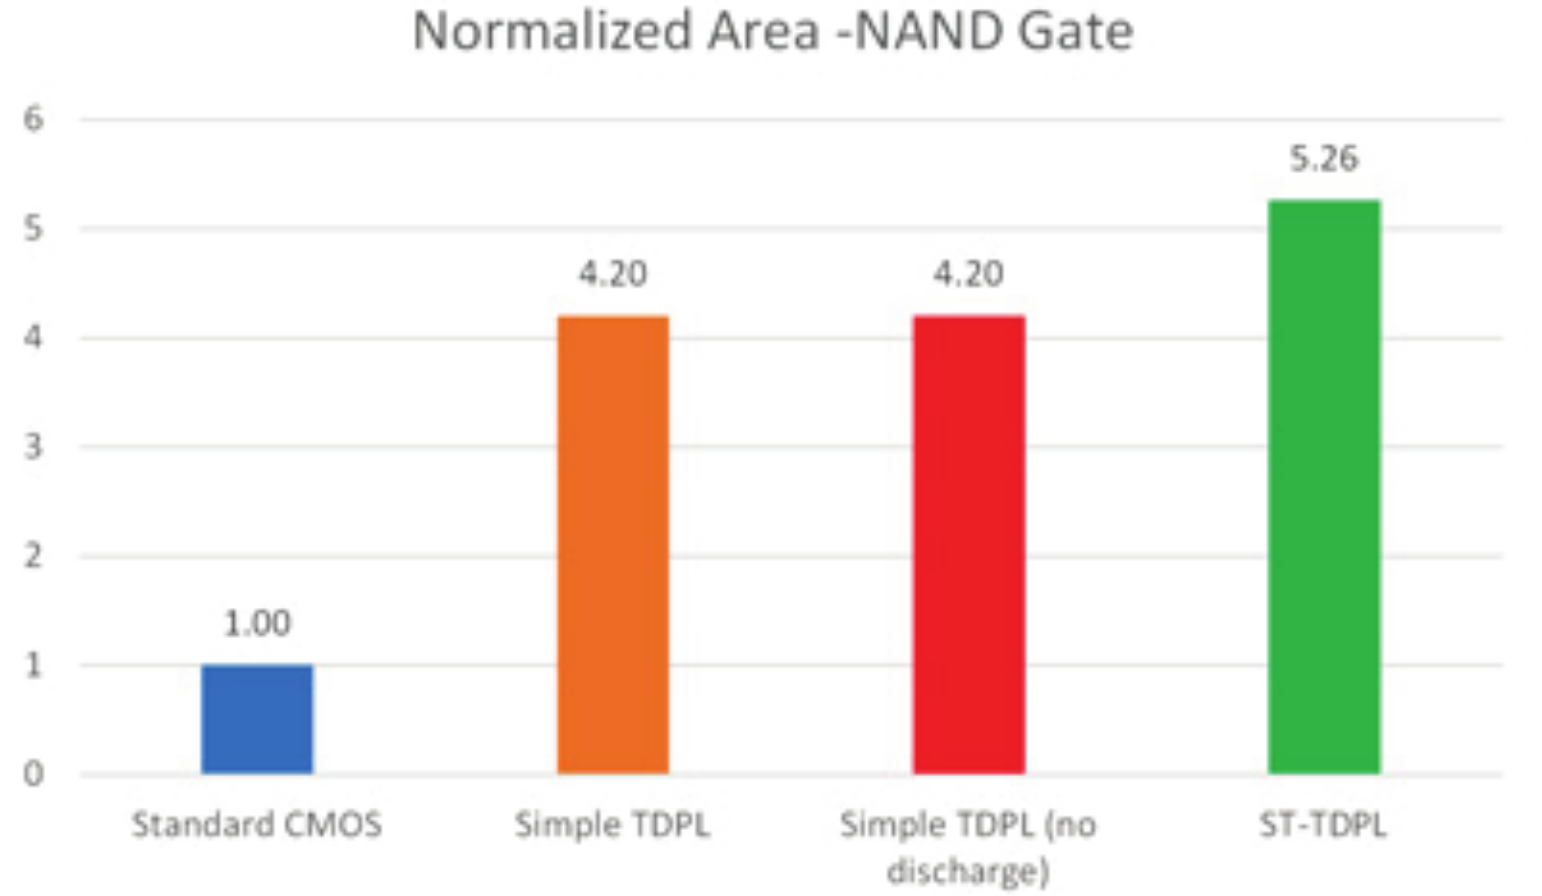
\includegraphics[width=\x\linewidth]{ReportFiles/ST-TDPL_Area.png}
				\caption{NAND gate area for CMOS, TDPL, compromised TDPL, and ST-TDPL.\cite{b2}}
				\label{ST-TDPL_Area}
			\end{figure}

		\subsection{Tunnel FETs}
			Along with traditional MOSFETs, there is some research into using emerging FET technology to reduce power consumption in DPA-resistant circuits. The most popular emerging technology in reducing power consumption is the Tunneling FET (TFET). The TFET has been shown to theoretically be a significant improvement over the MOSFET in terms of threshold voltage as well as subthreshold swing.

			In TFETs, the source and drain terminals are doped of the opposite type as shown in Figure \ref{TFET}. As gate bias is applied to the gate terminal, electron accumulation occurs in the intrinsic region between the two doped regions. Once the gate bias reaches a sufficient threshold, band-to-band tunneling occurs. Tunneling is a quantum process wherein electrons pass through potential energy barriers. In band-to-band tunneling, electrons tunnel through the band gap between the valence band and the conduction band of the two doped regions. 

			\begin{figure}[tbp]
				\centering
				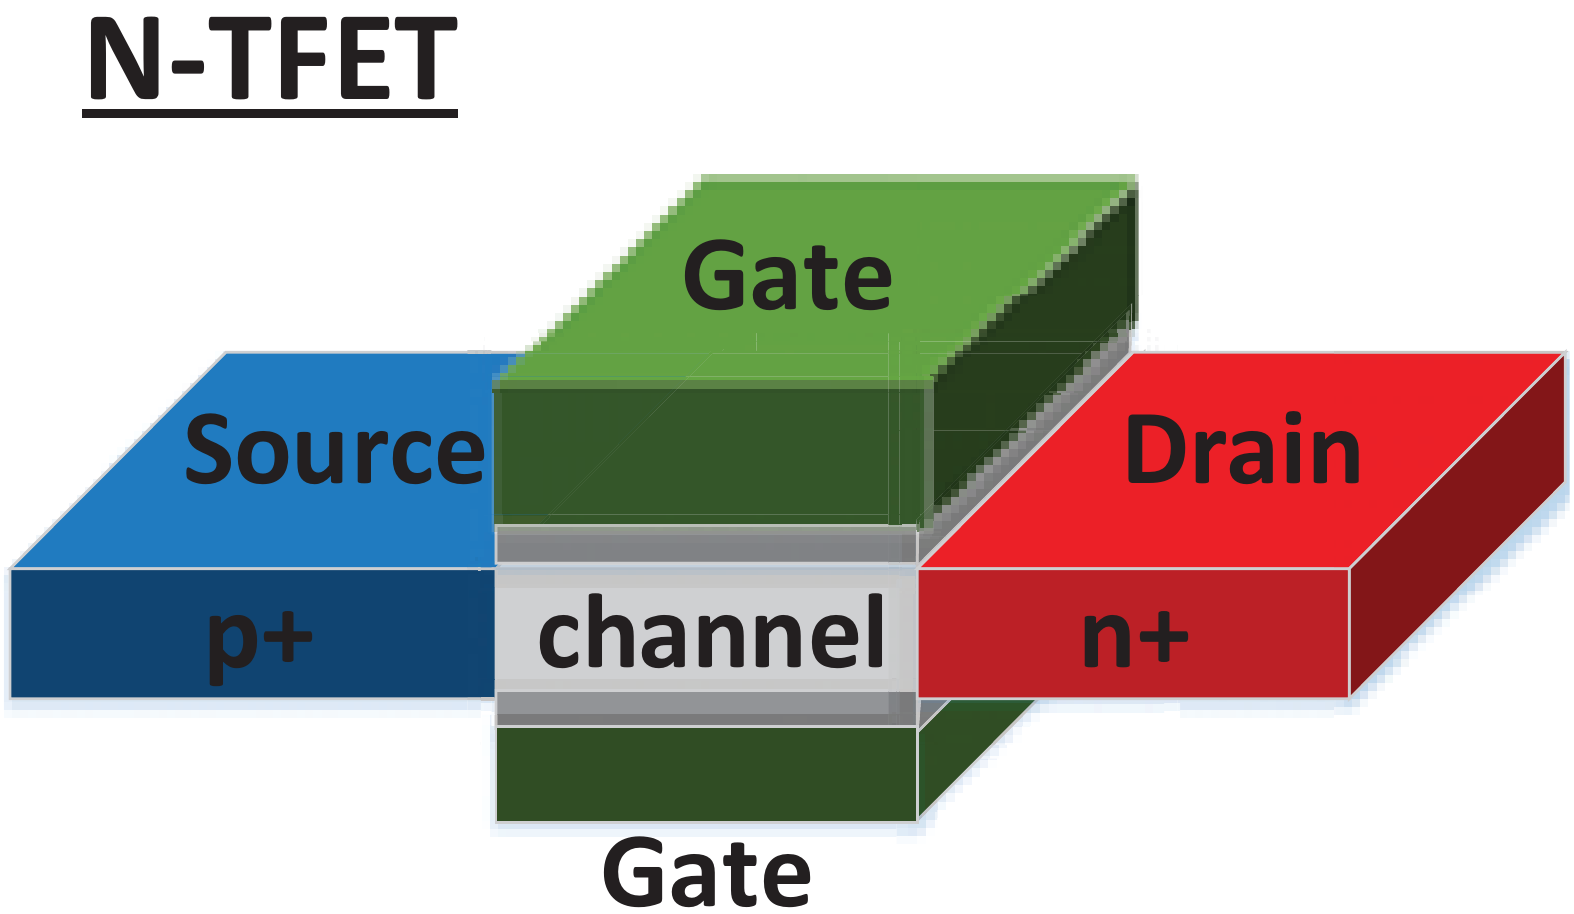
\includegraphics[width=\x\linewidth]{ReportFiles/TFET.png}
				\caption{Physical structure of a Tunnel FET (TFET).\cite{b4}}
				\label{TFET}
			\end{figure}

			TFETs have been shown to be extremely low power devices with a subthreshold swing of as low as 40mV/dec compared to the lower bound of 61 mV/dec in MOSFETs. From this, the threshold voltage is significantly lower than with MOSFETs, allowing the TFETs to use the same drain current with a lower voltage, showing large power savings.

			In \cite{b3}, MOSFETs are replaced with TFETs in the Symmetric Pass Gate Adiabatic Logic (SPGAL) logic style. Adiabatic logic differs from differential logic in that it utilizes energy recovery logic to recycle charge stored in load capacitors through the use of power clocks. Storing the energy allows the circuit to operate with reduced dynamic switching energy. Figure \ref{Energy_Recovery} shows how energy recovery circuits operate through the charging and discharging of load capacitors while Figure \ref{SPGAL_Buffer} shows how this concept is used in designing an SPGAL buffer circuit along with a timing diagram for operation of the circuit. 

			\begin{figure}[tbp]
				\centering
				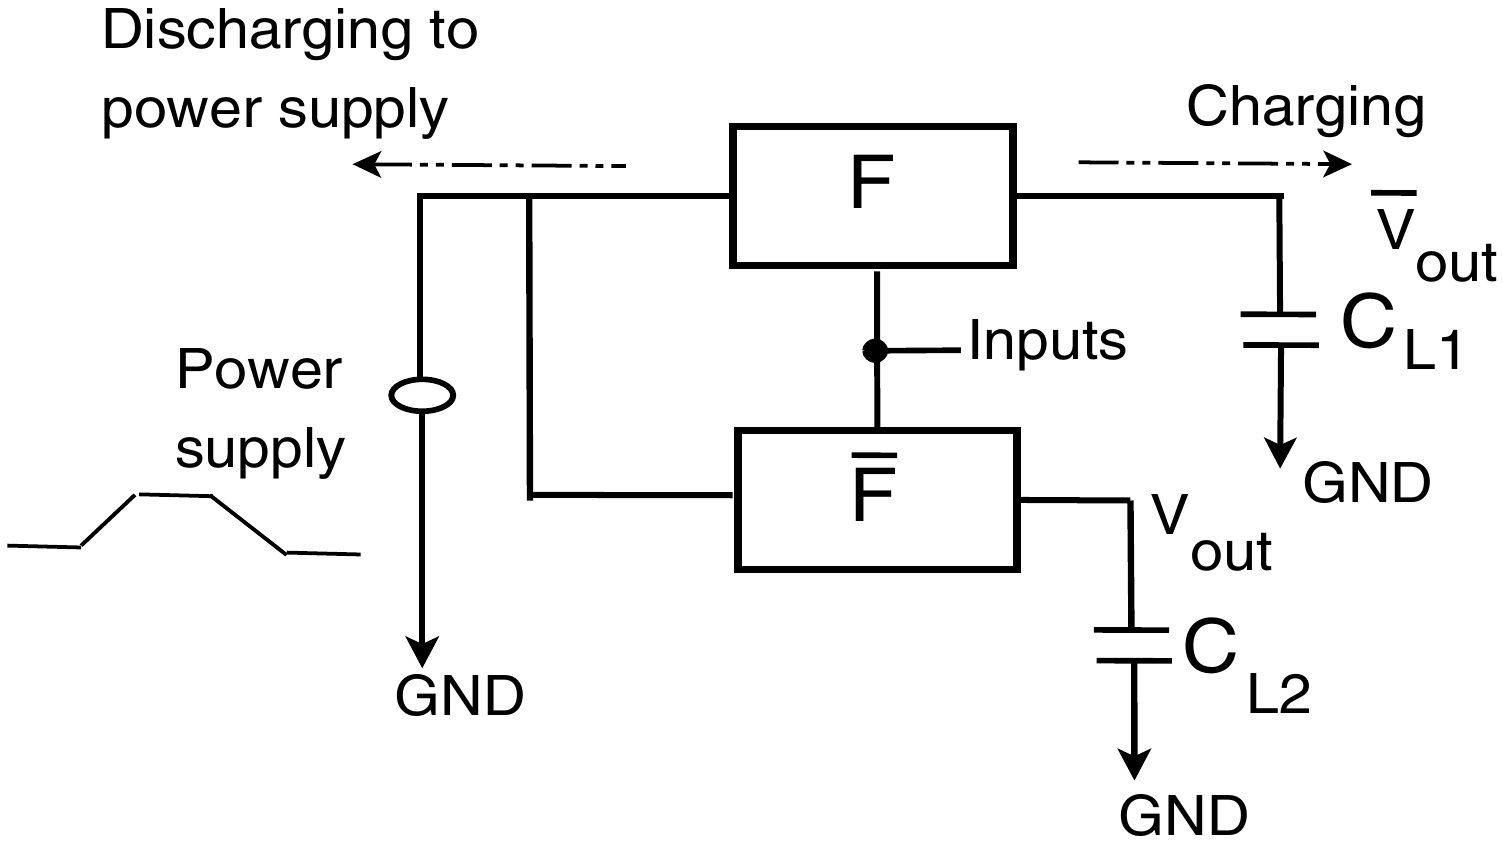
\includegraphics[width=\x\linewidth]{ReportFiles/Energy_Recovery.png}
				\caption{Energy recovery circuit operations using load capacitors.\cite{b3}}
				\label{Energy_Recovery}
			\end{figure}

			\begin{figure}[tbp]
				\centering
				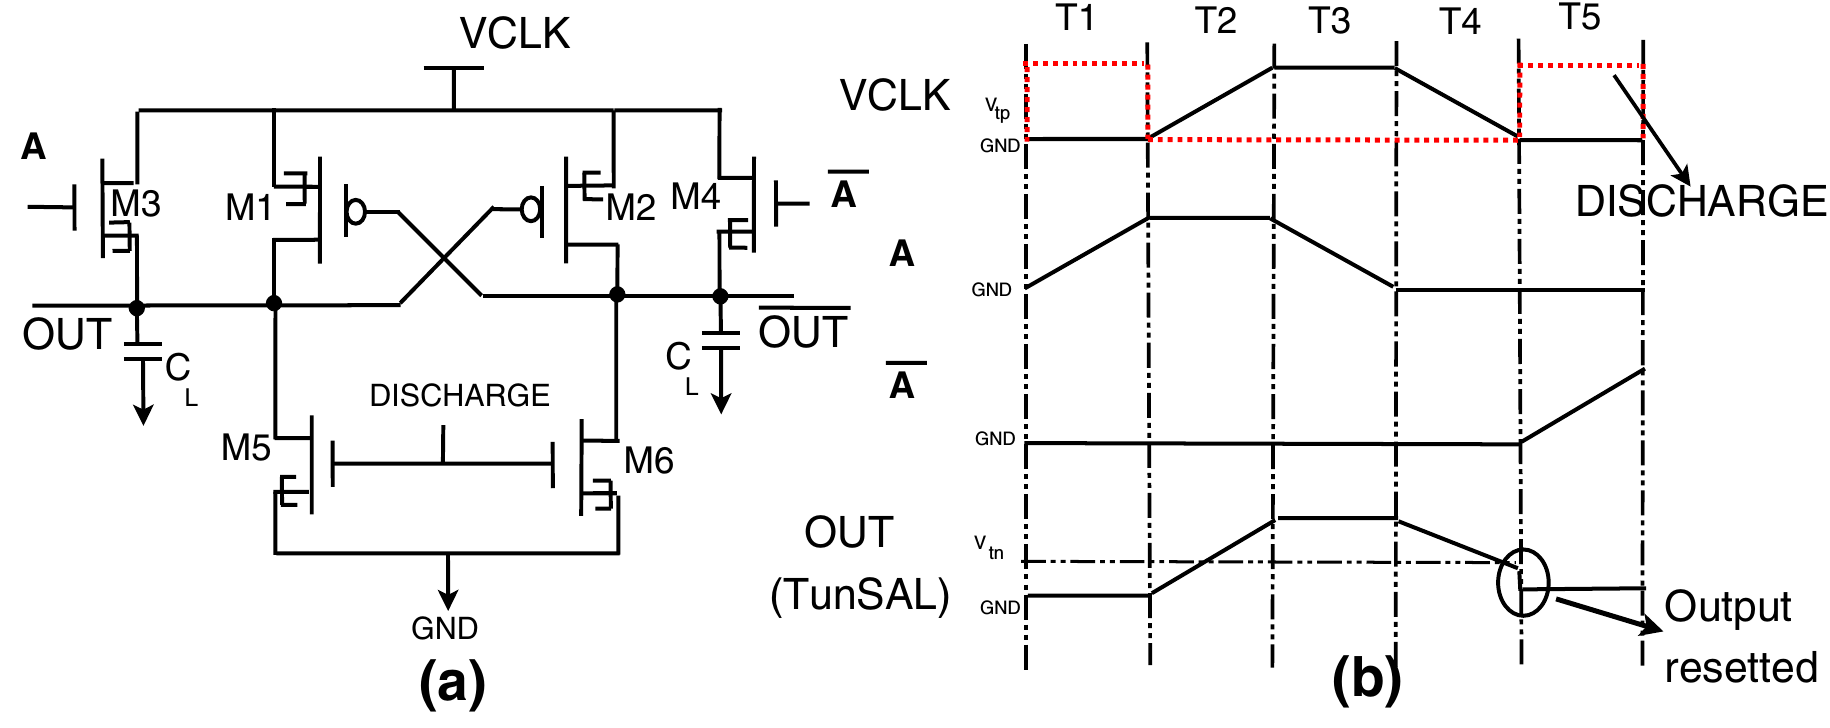
\includegraphics[width=\x\linewidth]{ReportFiles/SPGAL_Buffer.png}
				\caption{Energy recovery circuit usage in SPGAL buffer implementation with TFETs.\cite{b3}}
				\label{SPGAL_Buffer}
			\end{figure}

			The authors then perform simulations comparing CMOS- and TFET-based SPGAL circuits where the CMOS implementations use an input voltage of 1V and TFET implementations use an input voltage of 0.3V due to their lower threshold voltage. XOR gates are designed and simulated using Cadence Virtuoso. The results of these simulations show that the TFET implementation used an average of 0.045 fJ of energy while the MOSFET implementation used an average of 0.267 fJ for a decrease of 83\% energy usage when using TFETs over MOSFETs. 

			To test the TFET power savings in a realistic application, the lightweight cryptography (LWC) algorithm Present-80 is implemented using TFET- and CMOS-based SPGAL circuits. The energy measurements in this application for the CMOS implementation is 3.564 pJ and the power usage is \SI{1.32}{\micro\watt}. For the TFET implementation, the energy usage is 1.257 pJ and the power usage is \SI{0.511}{\micro\watt}. This is a percent decrease of 64.7\% and 61.3\% in energy and power usage, respectively. This demonstrates that TFETs are a very promising avenue for significant power savings over not only standard CMOS gates, but also DPA-resistant, energy-recovering CMOS gates.

			In \cite{b4}, TFETs are used in place of MOSFETs in the Current Mode Logic (CML) logic style. CML is designed to consume constant power throughout operation by applying constant current to the circuit. An added benefit of CML logic designs is an extremely fast switching speed to reduce switching power. A CML design operates with a tail transistor in the pull-down network that acts as a current source. Based on the input values, the current is sent up through an unbalanced NMOS-tree in the pull-down network. The current then goes through the pull-up network, causing the output in the same branch to go low while the other output is left high. Figure \ref{CML_TFET_XOR} shows an XOR gate implementation using CML logic with TFET transistors.

			\begin{figure}[tbp]
				\centering
				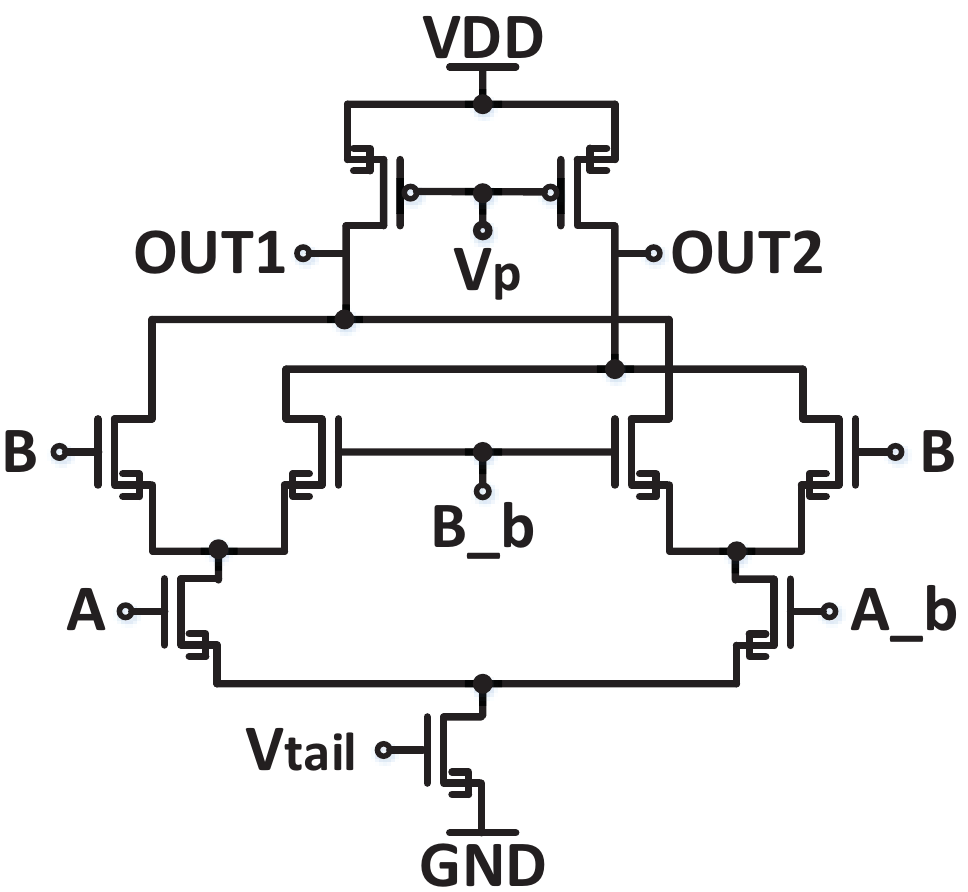
\includegraphics[width=\x\linewidth]{ReportFiles/CML_TFET_XOR.png}
				\caption{Current Mode Logic implementation of XOR gate using TFETs.\cite{b4}}
				\label{CML_TFET_XOR}
			\end{figure}

			As with the previous simulations from \cite{b3}, the authors of \cite{b4} examine the power reducing ability of TFETs with a lower threshold voltage. Additionally, the switching delay time is tested as CML can reduce this value significantly. Figure \ref{TFET_CML_Power} shows the results of average power and delay measurements for buffer, OR, AND, MUX, XOR, and D Flip Flop circuits implemented using CML logic style with TFET transistors. From this, it can be seen that the power usage is in the range of 25 to 50 nW. To prove the DPA-resistance of CML with TFETs, Figure \ref{TFET_CML_XOR_Power} shows the power traces for the XOR implementation with static and CML logic styles. This trace shows that the output power of CML is significantly more constant with a lower deviation than the standard static implementation using TFETs. 

			\begin{figure}[tbp]
				\centering
				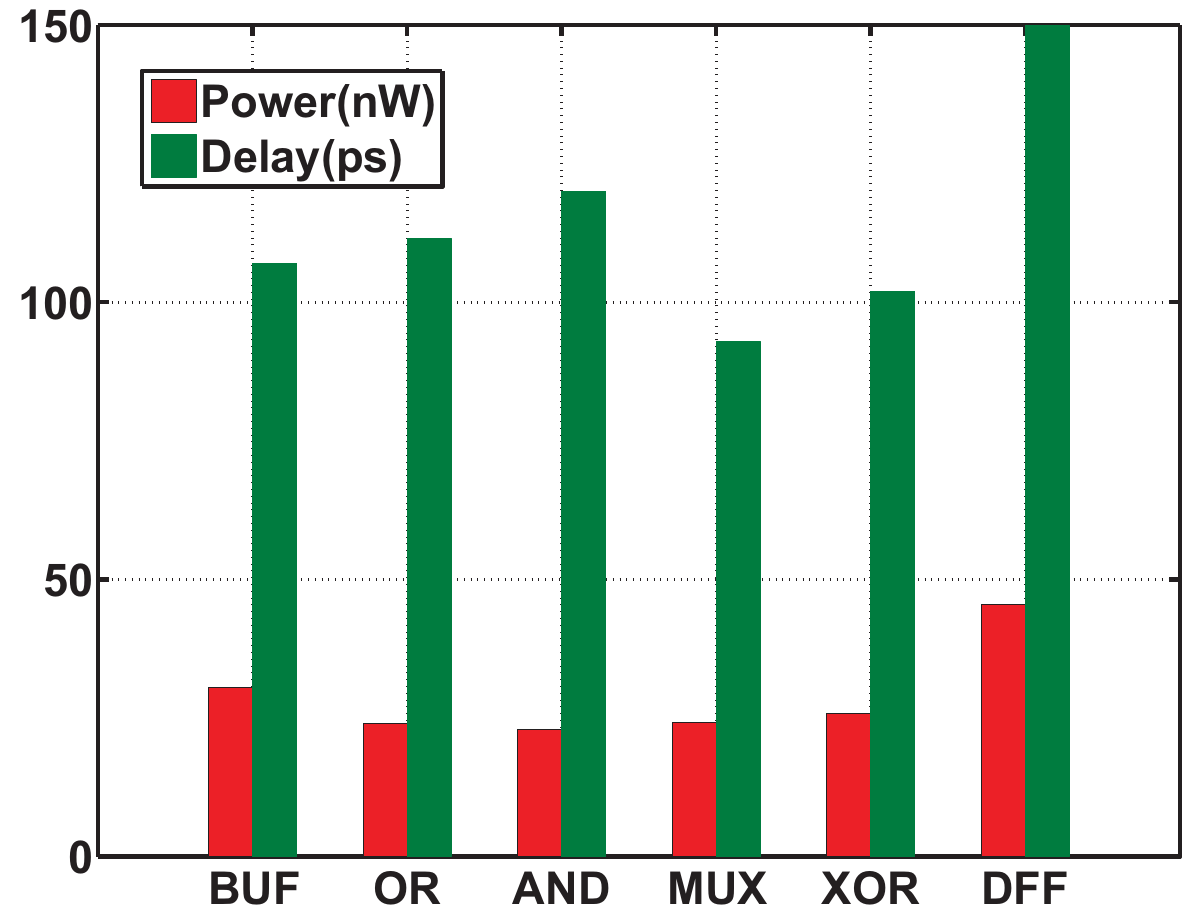
\includegraphics[width=\x\linewidth]{ReportFiles/TFET_CML_Power.png}
				\caption{Average power measurements for various CML TFET gates.\cite{b4}}
				\label{TFET_CML_Power}
			\end{figure}
			\begin{figure}[tbp]
				\centering
				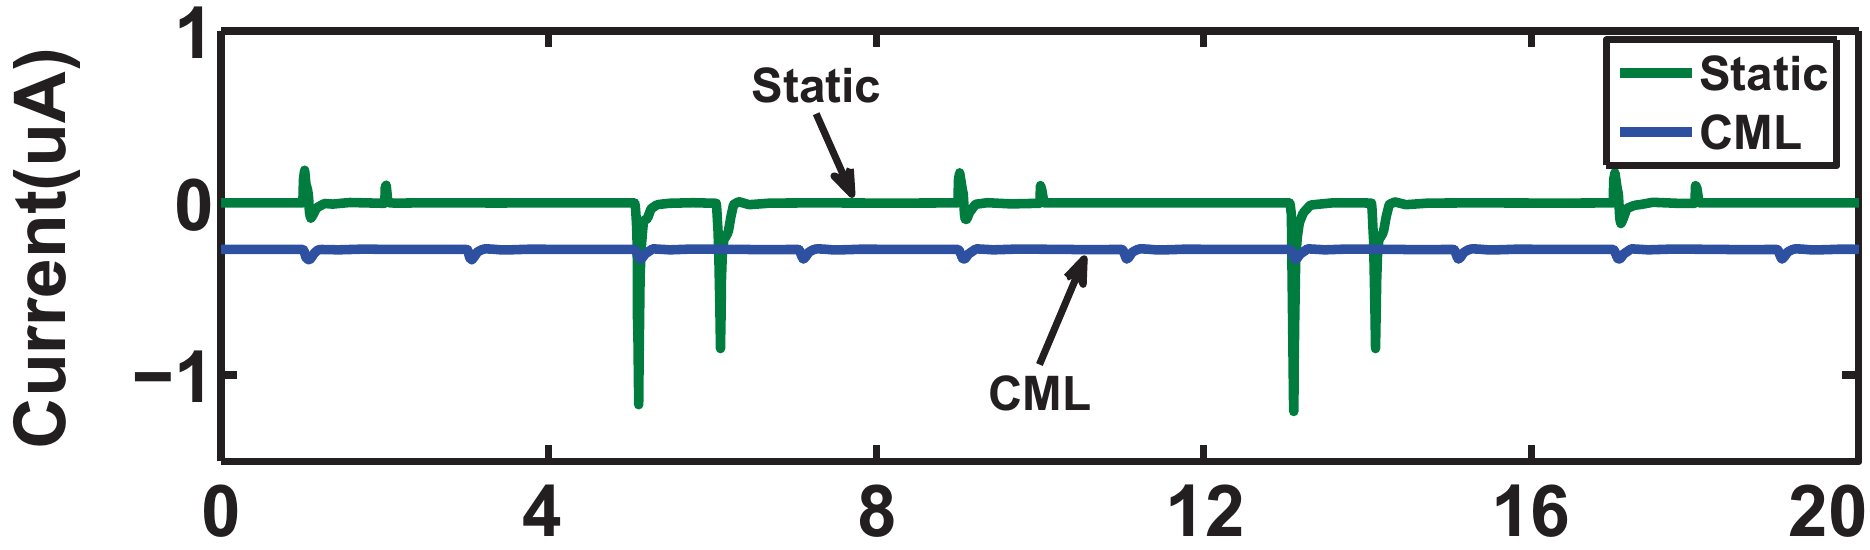
\includegraphics[width=\x\linewidth]{ReportFiles/TFET_CML_XOR_Power.png}
				\caption{Power output deviation of static versus CML TFET XOR gate implementation.\cite{b4}}
				\label{TFET_CML_XOR_Power}
			\end{figure}

		\subsection{Differential Pull-Down Network Improvements}
			Reference \cite{b5} proposes improvements to the differential pull-down network (DPDN) used in many logic styles. The proposed improvements are intended to work with any pull-up network and thus with any logic style. The first proposed improvement is the elimination of stored charges in internal nodes in order to avoid harmful memory effects leading to information leakage causing circuits to no longer be DPA-resistant. This effect can be seen in Figure \ref{SABL_XOR_Reference}. This figure shows the timing diagram of a SABL NAND/AND implementation. The waveforms for the $n1$ and $n2$ nodes can be seen to have differing stored charges at each clock cycle. During operation, this causes information leakage, causing DPA attacks to be successful

			\begin{figure}[tbp]
				\centering
				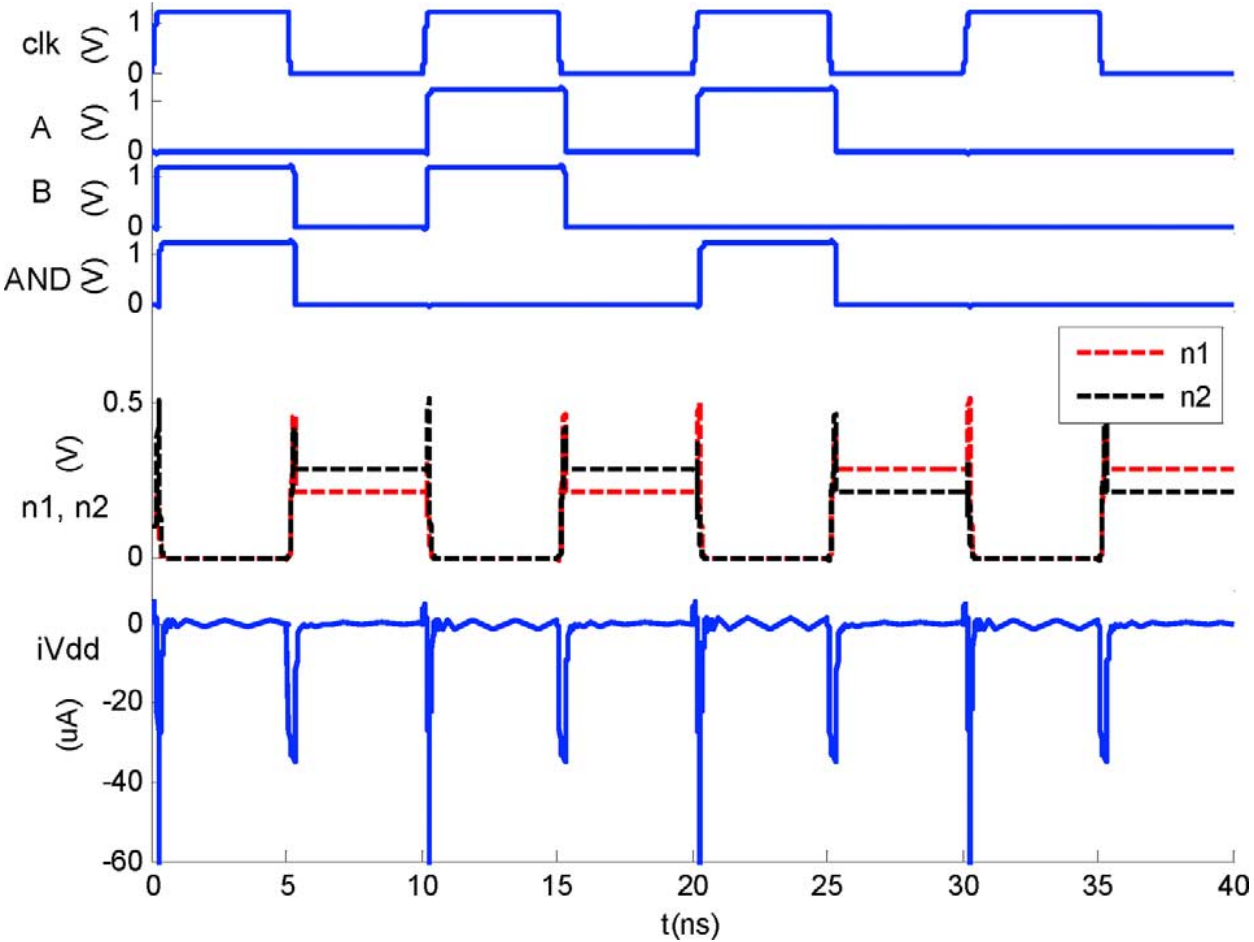
\includegraphics[width=\x\linewidth]{ReportFiles/SABL_XOR_Reference.png}
				\caption{Classic SABL timing diagram for XOR. Note the differences of the $n1$ and $n2$ nodes.\cite{b5}}
				\label{SABL_XOR_Reference}
			\end{figure}

			To remove stored charge in internal nodes, the proposed DPDN attempts to match the charge between the nodes in the pre-charge phase of operation. This can be done by either recycling the charge stored in the nodes, or by simply charging or discharging them all to a final value. The first solution to this problem is to add a single switch transistor for each level in the DPDN. This solution is shown in Figure \ref{DPDN_NAND_1Switch} which displays a DPDN for a NAND/AND gate with the switch PMOS transistor connected between the two branches in the network. 

			\begin{figure}[tbp]
				\centering
				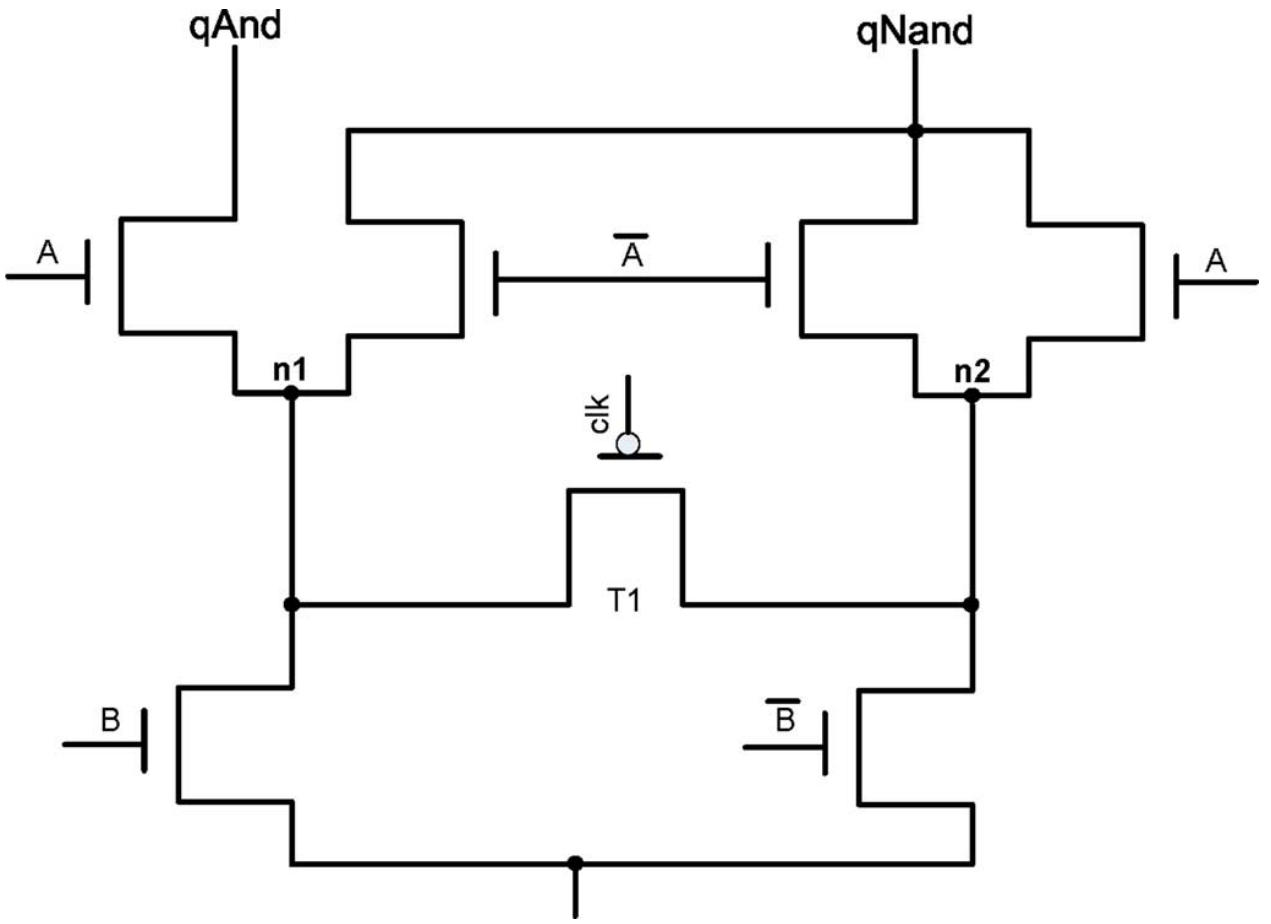
\includegraphics[width=\x\linewidth]{ReportFiles/DPDN_NAND_1Switch.png}
				\caption{Differential pull-down network showing the single switch case.\cite{b5}}
				\label{DPDN_NAND_1Switch}
			\end{figure}

			Thus, at each clock pulse, the two nodes $n1$ and $n2$ are charged or discharged when the clock is low or high, respectively. This effect is then shown in Figure \ref{DPDN_Single_Switch_Timing} which displays the corrected timing diagram from the implementation in Figure \ref{DPDN_NAND_1Switch}. The waveforms here for nodes $n1$ and $n2$ can be seen to be nearly equal the entire time, minimizing information leakage and improving the DPA-resistance of the circuit. 

			\begin{figure}[tbp]
				\centering
				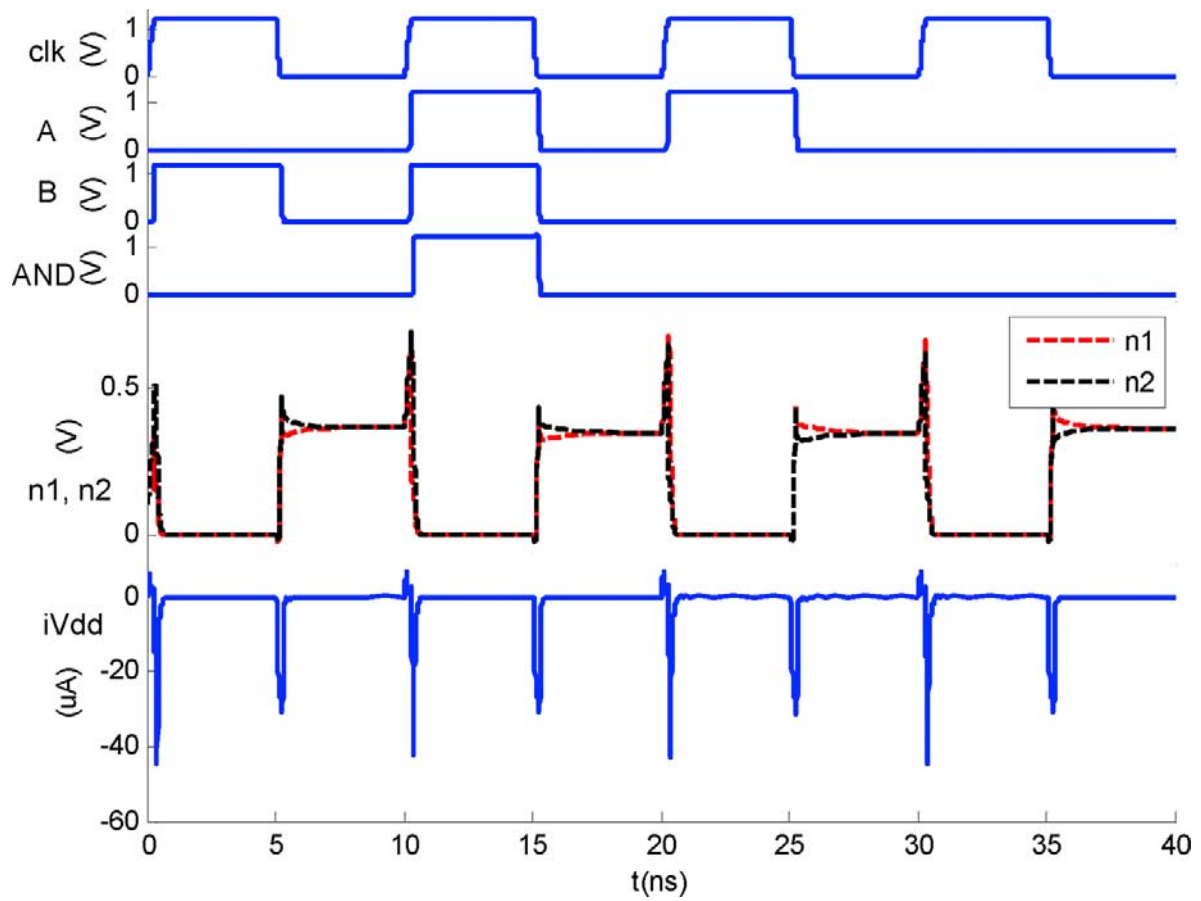
\includegraphics[width=\x\linewidth]{ReportFiles/DPDN_Single_Switch_Timing.png}
				\caption{Timing diagram for single switch solution to equally charge nodes $n1$ and $n2$.\cite{b5}}
				\label{DPDN_Single_Switch_Timing}
			\end{figure}

			To further improve the stored charge difference between the two nodes, a two-switch solution is also proposed. In this, a PMOS transistor is connected between each node and the source voltage (thus, two switches per level). Figure \ref{DPDN_NAND_2Switch} shows the proposed NAND/AND schematic with a clock-gated PMOS connected to $n1$ and another to $n2$. Figure \ref{DPDN_Two_Switch_Timing} then shows the timing diagram for this schematic. This continues to show improvements in charge matching between the two nodes. However, this doubles the extra area cost for the clock-gated transistors as well as the power consumption of the circuit, so this solution should only be considered in devices where power consumption is not necessarily more important than absolute security. 

			\begin{figure}[tbp]
				\centering
				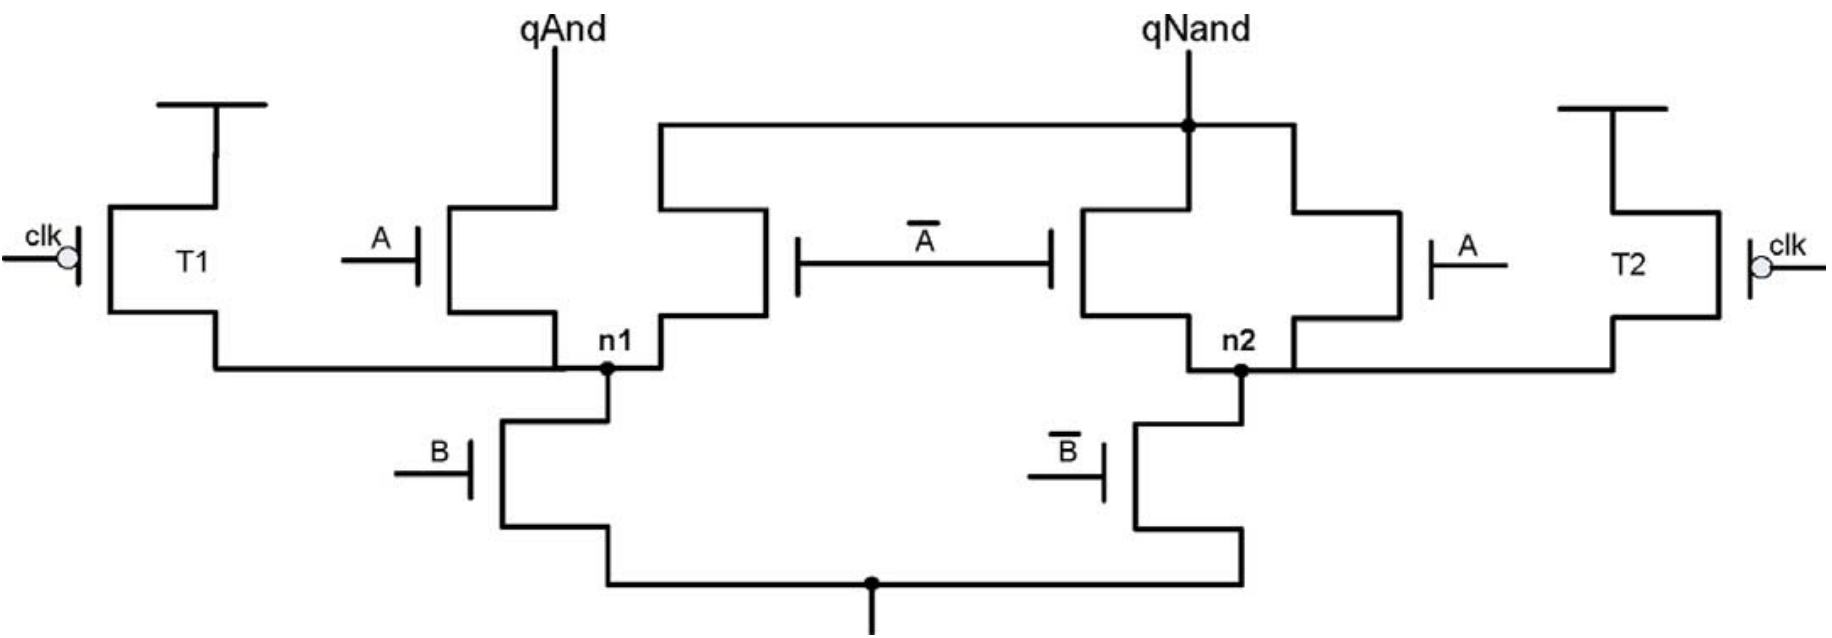
\includegraphics[width=\x\linewidth]{ReportFiles/DPDN_NAND_2Switch.png}
				\caption{Differential pull-down network for a NAND gate with the two switch proposal.\cite{b5}}
				\label{DPDN_NAND_2Switch}
			\end{figure}
			\begin{figure}[tbp]
				\centering
				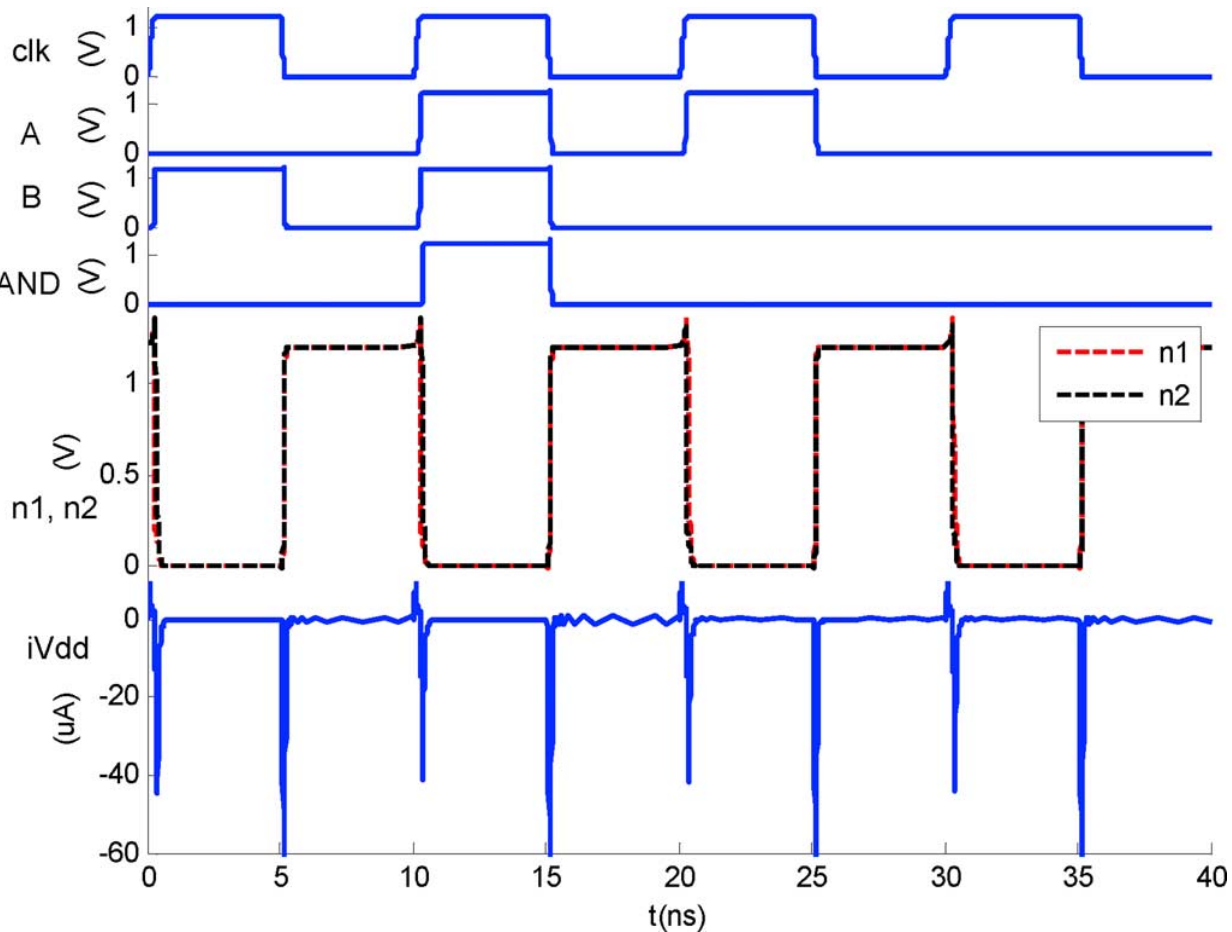
\includegraphics[width=\x\linewidth]{ReportFiles/DPDN_Two_Switch_Timing.png}
				\caption{Timing diagram for two switch solution to equally charge nodes $n1$ and $n2$ to $V_{DD}$.\cite{b5}}
				\label{DPDN_Two_Switch_Timing}
			\end{figure}

			To prove DPA-resistance, the authors then perform an Sbox9 case study. The Sbox9 case uses the 9-bit substitution box used in the Kasumi algorithm which is used in cellular communications. Three cases are examined for this study: standard cell, classic SABL, and the proposed implementation. To measure the results, the authors measure the Measurements to Disclosure (MTD). MTD represents the number of power traces need to be measured before the correct key is discovered. Figures \ref{Classic_MTD}, \ref{SABL_MTD}, and \ref{DPDN_MTD} show the plots of the correlation coefficients versus trace number for standard CMOS cell, SABL, and proposed implementations, respectively. From this, it can be seen that standard cell can be compromised in as little as 145 measurements and SABL is compromised in 344 measurements. After 10,000 input patterns, the proposed implementation is not compromised. This shows that the proposed implementation is extremely strong against DPA attacks and that, by adding switches to the circuit, almost perfectly secure DPA-resistance can potentially be achieved.

			\begin{figure}[tbp]
				\centering
				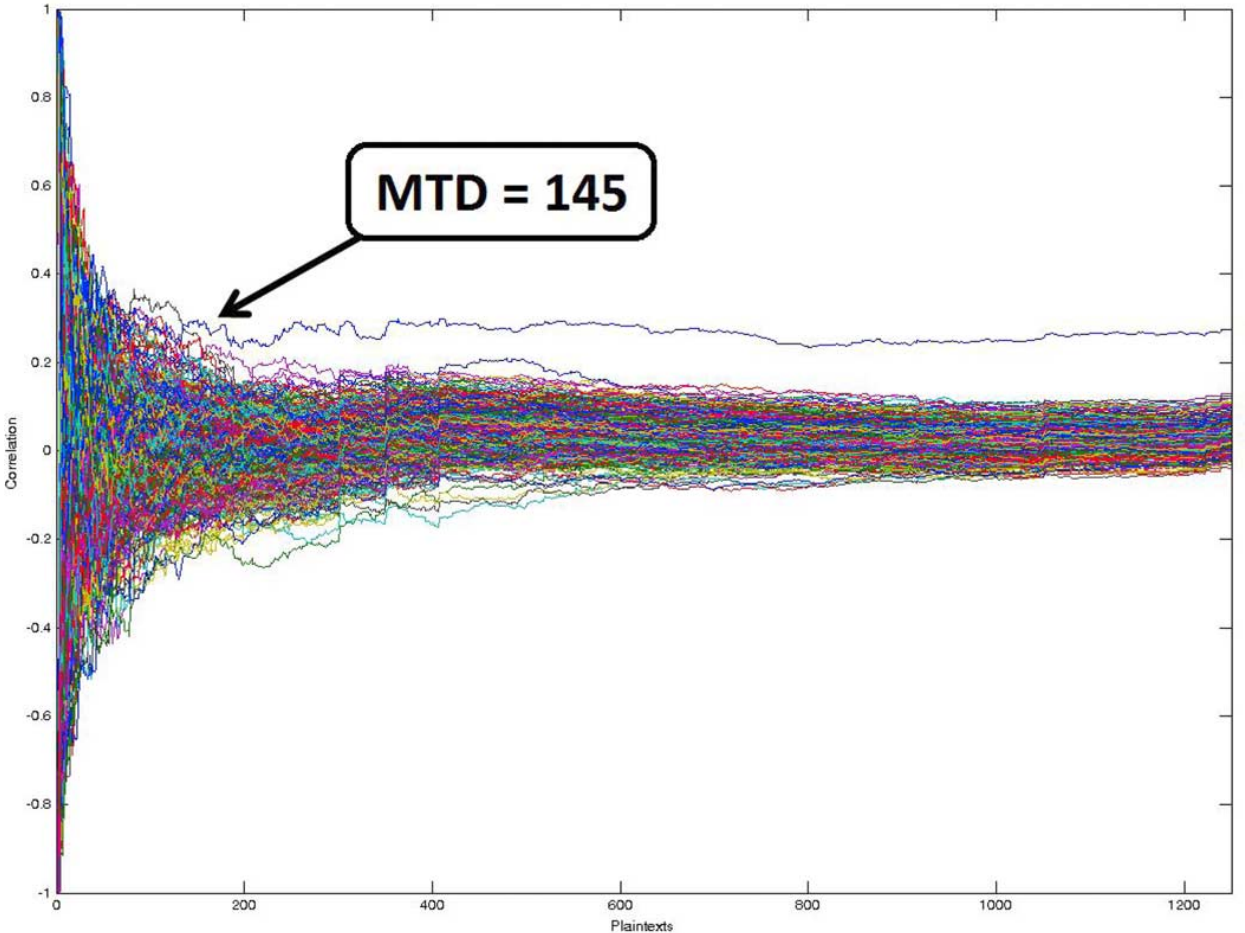
\includegraphics[width=\x\linewidth]{ReportFiles/Classic_MTD.png}
				\caption{Measurements to Disclosure plot of classic CMOS Sbox9 implementation.\cite{b5}}
				\label{Classic_MTD}
			\end{figure}
			\begin{figure}[tbp]
				\centering
				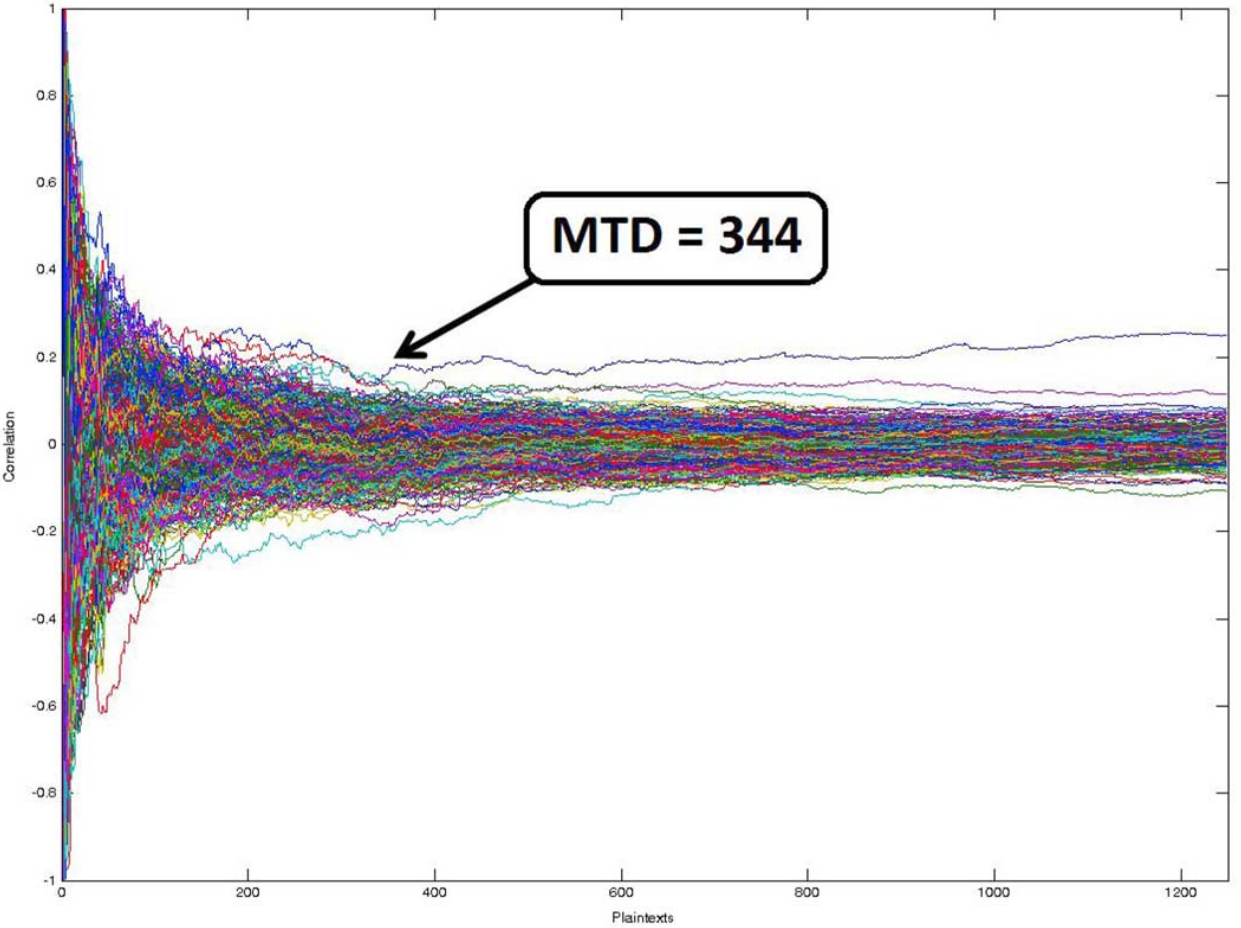
\includegraphics[width=\x\linewidth]{ReportFiles/SABL_MTD.png}
				\caption{Measurements to Disclosure plot of SABLE Sbox9 implementation.\cite{b5}}
				\label{SABL_MTD}
			\end{figure}
			\begin{figure}[tbp]
				\centering
				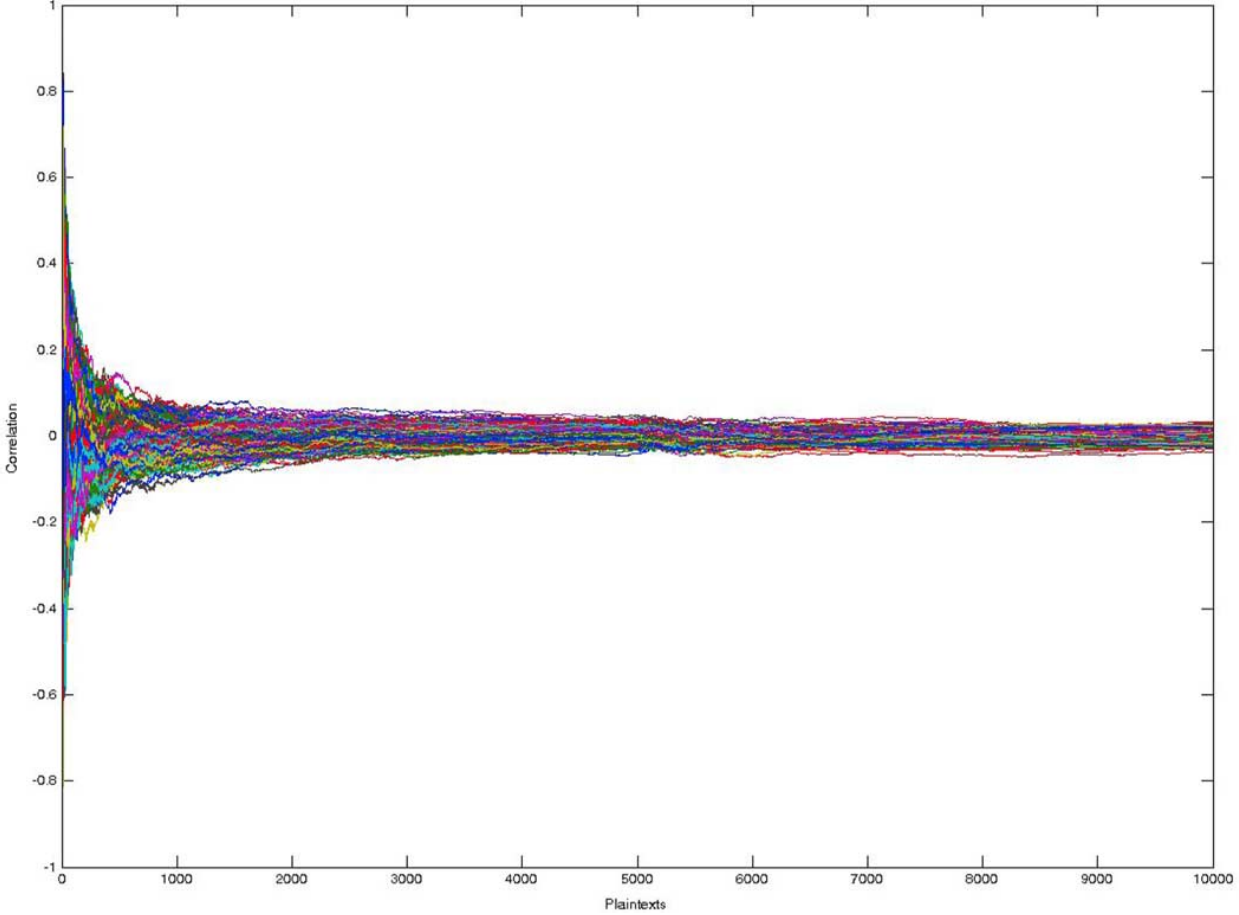
\includegraphics[width=\x\linewidth]{ReportFiles/DPDN_MTD.png}
				\caption{Measurements to Disclosure plot of SABLE Sbox9 implementation with proposed pull-down network.\cite{b5}}
				\label{DPDN_MTD}
			\end{figure}

		\subsection{Nano-Scale Differential Logic}
			Reference \cite{b6} attempts to combine characteristics from existing logic styles into a novel proposal with significantly reduced Normalized Energy Distribution (NED). With an increased NED, the number of traces needed for a DPA to successfully find a matching key also increases rapidly, increasing the difficulty for an adversary to successfully mount an attack.

			The proposed logic style uses the pre-charge and evaluation phases as well as the dual-rail characteristic from previous differential logic styles such as TDPL. The schematic for the proposed NAND/AND gate is shown in Figure \ref{Nano_NAND}. The input signal $\Phi$ represents the two phases of operation, 0 for pre-charge and 1 for evaluation phase and is sourced by the clock signal. During the pre-charge phase, the two output lines are set high. During the evaluation phase, the differential pull-up network is turned off and one branch from the pull-down network powers one output line high and the other low, dependent on the input values. 

			\begin{figure}[tbp]
				\centering
				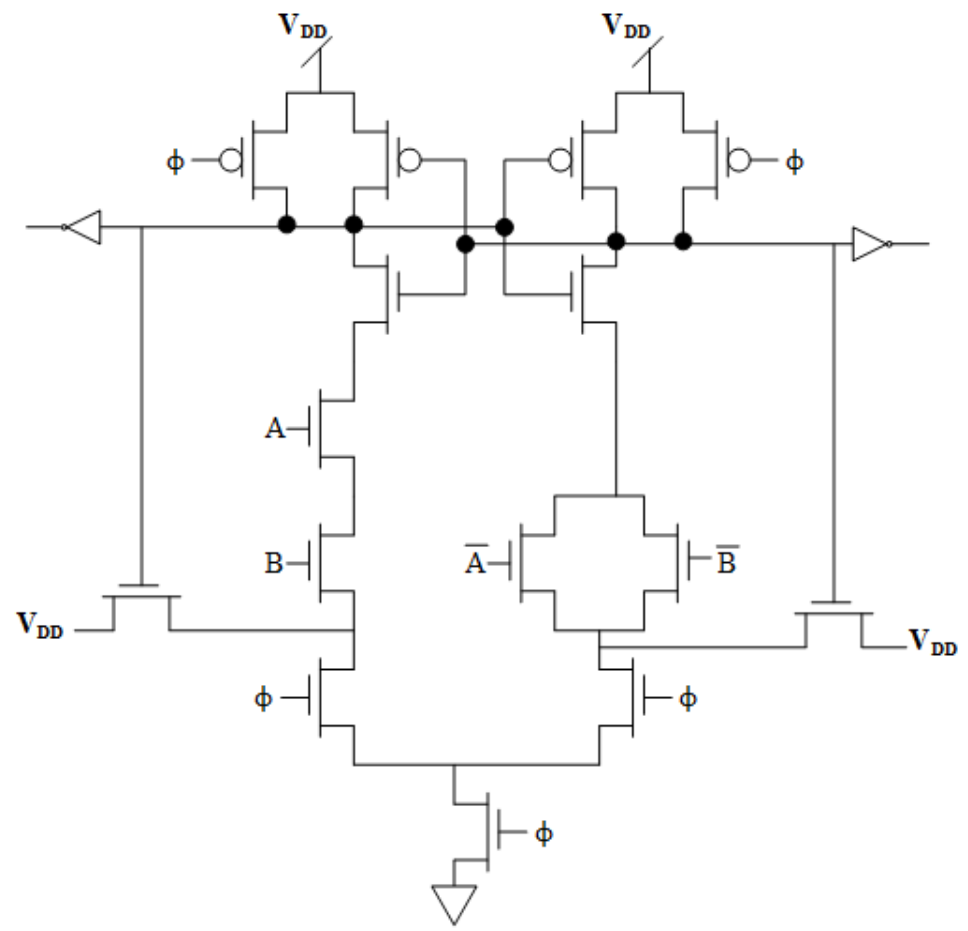
\includegraphics[width=\x\linewidth]{ReportFiles/Nano_NAND.png}
				\caption{Nano-Scale NAND gate implementation.\cite{b6}}
				\label{Nano_NAND}
			\end{figure}

			Because there is only one clock input, the power draw for these two phases is significantly less than implementations where multiple sources are needed and is comparable in power consumption to standard CMOS implementations. To reduce leakage current, the gates are designed such that there are more than three stacked transistors between the supply and ground in both NAND/AND and XOR/XNOR implementations. 

			To measure the power distribution requirements and DPA-resistance, HSPICE simulations are run comparing TDPL, Simple TDPL (STDPL), SABL, and 3sDDL with the proposed logic. While there is some extra area usage (15 transistors versus 11-14 for others) and maximum energy usage, the Normalized Energy Distribution (NED) is reduced down to 0.21\% for the NAND/AND implementation. Further, the NED for the XOR/XNOR implementation is reduced to 0.23\%. This is a significant value as 1\% is generally considered acceptable security against DPA attacks. Thus, the proposed nano-scale differential logic is extremely robust against DPA attacks. 

			During most simulations, balanced capacitance loads are applied. However, this is not always the case in real-world applications. In this paper, the authors considered this and ran simulations testing capacitance mismatch conditions of 200\% and 300\% (typical of dual-rail logics). The results of this test show that the proposed logic maintains its ability to produce a very low NED as shown in Figure \ref{Nano_Mismatched_Capacitance}. This graph compares the NED results for all tested logic styles using NAND gates with a 200\% and 300\% capacitance mismatch. Despite the decrease in NED for all cases, the overall power consumption of the proposed logic is extremely high compared to other implementations. While the TDPL NAND gate is measured at a maximum energy usage of 4.62 fJ, NAND gates in the proposed logic style are measured at a maximum energy of 113 fJ, an increase of nearly 25 times. Thus, this proposed logic style should only be used in applications where power is not a primary concern.

			\begin{figure}[tbp]
				\centering
				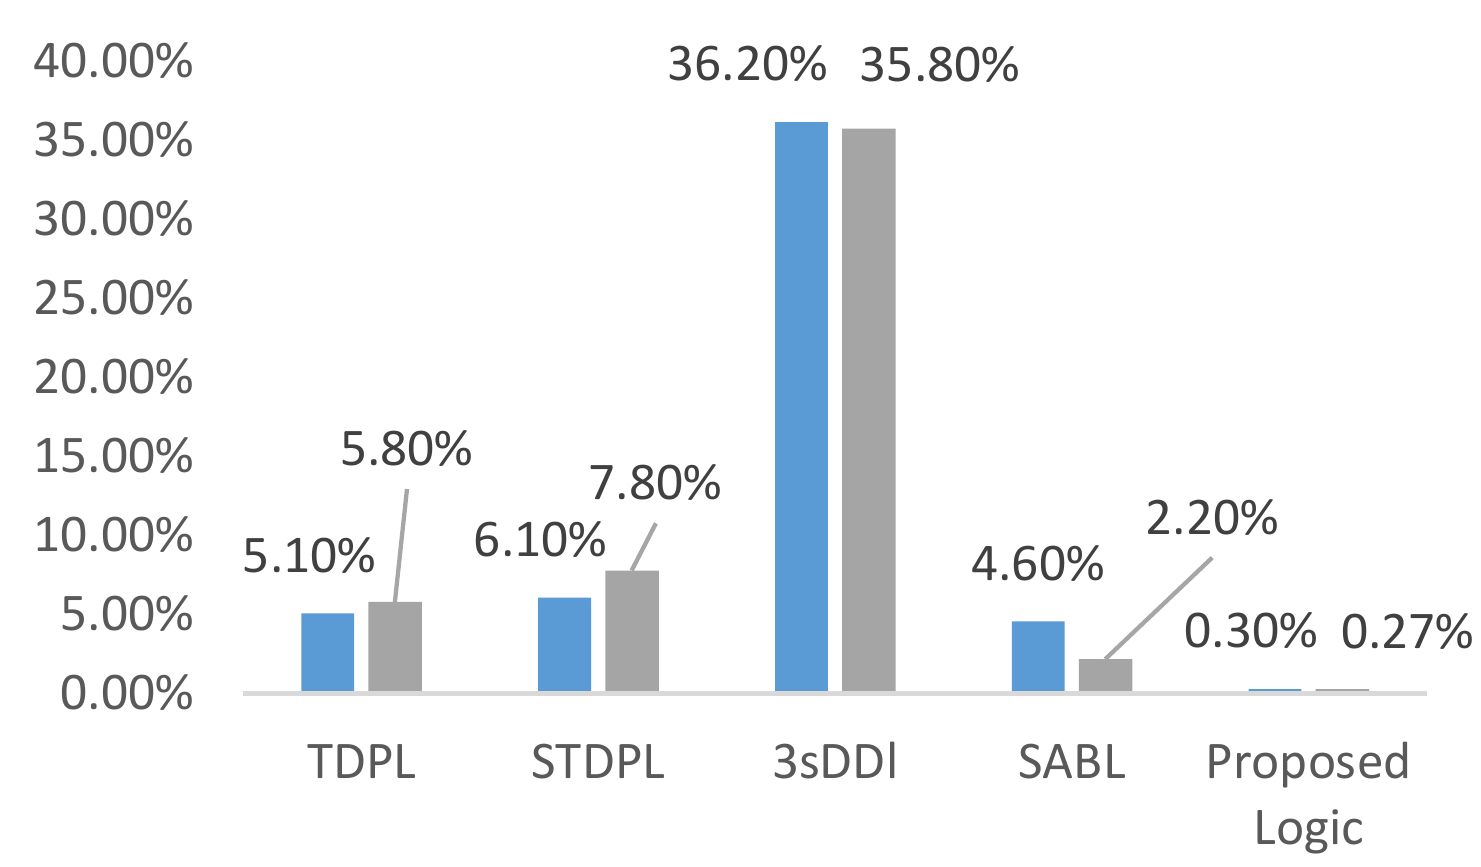
\includegraphics[width=\x\linewidth]{ReportFiles/Nano_Mismatched_Capacitance.png}
				\caption{Normalized energy deviation values for NAND gates when capacitance mismatch is 200\% (blue) and 300\% (gray).\cite{b6}}
				\label{Nano_Mismatched_Capacitance}
			\end{figure}

	\section{Comparisons of Proposed Logic Styles}
		Despite all having the same main goal, it can be very difficult to directly compare two proposed logic styles. This is mainly due to the solutions being somewhat implementation-based as each proposed style is examined using a different algorithm and the results are interpreted differently. Despite this, some comparisons can still be drawn and some recommendations for usage can be made.

		In \cite{b1} and \cite{b2}, TDPL is measured against DPA attacks with the logic of \cite{b2} being named ST-TDPL as it is a self-timed version of the standard TDPL proposed in \cite{b1}. ST-TDPL is shown to take approximately 25\% more area than standard TDPL implementations. Despite this extra area and transistor requirement, ST-TDPL shows great improvements in energy consumption with a 34.9\% decrease in NAND and 31.8\% decrease in XOR energy consumption over TDPL. The normalized energy deviation of the NAND and XOR gates show a 33.3\% and 14.4\% decrease, respectively. Together, this shows that ST-TDPL is a great improvement in energy and DPA-resistance over standard TDPL with only a marginal area overhead. 

		References \cite{b3} and \cite{b4} explore the usage of Tunnel FETs (TFETs) in Symmetric Pass Gate Adiabatic Logic (SPGAL) and Current Mode Logic (CML), respectively. Both papers focus on the implementation of the XOR gate. While a direct comparison cannot be made due to the first measuring power and the latter measuring energy usage, it can be inferred that the energy recovery logic shown in \cite{b3} with the SPGAL implementation saves significant amounts of energy consumption. This is shown in the average energy used by the XOR gate, 0.045 fJ. Additionally, the Normalized Energy Distribution (NED) of this implementation is calculated as 0.00014\%, showing a near perfect DPA-resistance. 

		However, this only serves to prove that a single gate is DPA-resistant. In \cite{b3}, a lightweight cryptographic algorithm is implemented and measured to prove that, after 50,000 power traces, a DPA attack could not reveal the secret key. In \cite{b4}, no such implementation is examined. Given this, it appears that the SPGAL implementation using TFETs is both more secure, and slightly lower power usage due to the energy recovery design. Additionally, the TFET implementations show lower power usage than traditional CMOS logic, thereby showing that they are also more power efficient than other logic styles such as TDPL, SABL, and others. It can then be concluded that for ultra low-power considerations, TFETs, once available for large scale production, appear to be the best option to use regardless of the logic style being used.

		The final two proposals of \cite{b5} and \cite{b6} both attempt to improve the efficiency of Differential Pull-Down Networks (DPDNs). Therefore, they can potentially be included alongside the previous proposed logic styles as a further improvement. This, of course, does need to be examined first. In \cite{b5}, clock gated PMOS transistors are added as switches in two cases: one-switch and two-switch. In \cite{b6}, extra transistors are added to reduce leakage current by stacking transistors in branches between the source and ground. While both implementations generate impressive improvements in NED, the clock-gated implementation of \cite{b5} shows only a marginal increase in power while the nano-scale differential logic implementation of \cite{b6} shows a power increase of 25 times that of TDPL implementations. Thus, unless the implementation does not care at all about power, the clock-gated DPDN improvement is significantly more appealing. 

		In most applications, differential logic is the most secure gate implementation. Unless the power constraint of a device is in the narrow gap between TDPL and ST-TDPL implementation, ST-TDPL is generally the best tradeoff between power and security against DPA attacks. If extra power can be used, then the clock-gated implementation of \cite{b5} appears to be a good area and power investment. However, the DPA-resistance of ST-TDPL is more than enough for most applications (with the notable exception of high-security fields such as government and military). If mainstream TFET production becomes feasible, then replacing MOSFETs in these designs with TFETs does appear, based on the limited research, to be the best method of saving power due to the significantly lower threshold voltages required. 

	\section{Conclusion}
		In most mobile or IoT applications, TDPL or ST-TDPL will generally be secure and lightweight enough to both counter DPA attacks and not drain low-power devices. In less lightweight applications, ST-TDPL with the improvements of \cite{b5} appear to be enough to almost guarantee perfect security over an extremely large number of power traces for a DPA attack. If manufacturing precision is able to improve far enough, replacing MOSFETs with TFETs will show significant power savings in most or all applications. Future work in this area is needed to ensure that the proposed logic styles will work for the most popular cryptographic schemes such as Kasumi and Snow-3G in mobile applications as well more powerful algorithms and hash functions for larger devices.

	\begin{thebibliography}{00}
		\bibitem{b1} C. Satish Kumar, A. Prathiba, V.S. Kanchana Bhaskaran. ``DPA Resistance Analysis of the Cryptographic S-box Implementation in Static CMOS and TDPL Logic Style,'' in \textit{Proceedings of International Conference on Nextgen Electronic Technologies: Silicon to Software (ICNETS2)}, 23-25 March, 2017, pp. 281-288.
		\bibitem{b2} N. E. C. Akkaya, B. Erbagci, R. Carley, K. Mai. ``A DPA-resistant self-timed three-phase dual-rail pre-charge logic family,'' in \textit{Proceedings of IEEE International Symposium on Hardware Oriented Security and Trust (HOST)}, 5-7 May 2015, pp. 112-117.
		\bibitem{b3} H. Thapliyal, T. S. S. Varun, S. D. Kumar, ``Low-power and secure lightweight cryptography via TFET-based energy recovery circuits,'' in \textit{IEEE International Conference on Rebooting Computing}, 8-9 Nov. 2017, pp. 34-37.
		\bibitem{b4} K. Shamsi, W. Wen, Y. Jin, ``Hardware security challenges beyond CMOS: attacks and remedies,'' in \textit{Proceedings of IEEE Computer Society Annual Symposium on VLSI (ISVLSI)}, 11-13 July 2016, pp. 200-205.
		\bibitem{b5} E. T. Sánchez, J. Castro, A. J. Costa, ``A methodolgy for optimized design of secure differential logic gates for DPA resistant circuits,'' in \textit{IEEE Journal on Emerging and Selected Topics in Circuits and Systems}, vol. 4, no. 2, Jun., pp. 203-215, 2014.
		\bibitem{b6} A. Abdi, A. Jahanian, ``A new nano-scale differential logic style for power analysis attack,'' in \textit{Proceedings of 23rd Iranian Conference on Electrical Engineering (ICEE)}, 10-14 May 2015, pp. 584-588/
		\bibitem{b7} P. Kocher, J. Jaffe, B. Jun, ``Differential power analysis,'' in \textit{Proceedings of the 19th Annual International Cryptology Conference on Advances in Cryptology}, 15-19 August 1999, pp. 389-397.
	\end{thebibliography}
\end{document} 
